\chapter{Deuteronomio}


\section*{Introducción al Libro de Deuteronomio}

El \textbf{Deuteronomio} es el quinto y último libro del Pentateuco, considerado una obra fundamental tanto en la tradición judía como en la cristiana. Su título proviene del griego \textit{Deuteronomion}, que significa "segunda ley", haciendo referencia a la reiteración y explicación de la ley mosaica contenida en los libros anteriores. En hebreo, se le conoce como \textit{Devarim} ("Palabras"), ya que comienza con el discurso de Moisés al pueblo de Israel.

\subsection*{Autoría}

La tradición atribuye la autoría del Deuteronomio a \textbf{Moisés}, quien habría pronunciado y registrado sus discursos antes de la entrada del pueblo de Israel en la Tierra Prometida. Sin embargo, estudios modernos sugieren que el Deuteronomio es producto de una tradición literaria conocida como la escuela deuteronomista, cuya composición final habría tenido lugar durante el siglo VII a.C., en el contexto de las reformas religiosas del rey Josías, y fue ampliada en el período del exilio babilónico.

\subsection*{Temática}

El Deuteronomio está estructurado como un discurso final de Moisés al pueblo de Israel, exhortándolos a la obediencia y fidelidad al pacto con Dios. Sus temas principales incluyen:
\begin{itemize}
	\item \textbf{Recordatorio histórico} (Deuteronomio 1–4): Moisés recuerda los eventos del éxodo y la travesía por el desierto, subrayando la fidelidad de Dios.
	\item \textbf{Repetición de la Ley} (Deuteronomio 5–26): Incluye los Diez Mandamientos y una serie de leyes que regulan la vida religiosa, social y moral del pueblo.
	\item \textbf{Bendiciones y maldiciones} (Deuteronomio 27–28): Moisés advierte sobre las consecuencias de la obediencia o desobediencia al pacto.
	\item \textbf{Renovación del pacto} (Deuteronomio 29–30): Moisés llama al pueblo a renovar su compromiso con Dios antes de entrar en la Tierra Prometida.
	\item \textbf{La muerte de Moisés} (Deuteronomio 31–34): Relata el nombramiento de Josué como sucesor de Moisés y la muerte de este último en el Monte Nebo, desde donde observa la Tierra Prometida.
\end{itemize}



El Deuteronomio tiene una profunda conexión histórica con las reformas religiosas de Israel. Su énfasis en la centralización del culto en un único santuario y en la exclusividad de la adoración a Yahvé refleja los desafíos que enfrentaba el pueblo de Israel para mantenerse fiel en medio de influencias culturales y religiosas externas. Además, sus mensajes de esperanza y renovación eran especialmente significativos durante el exilio babilónico, cuando el pueblo enfrentaba el desafío de preservar su identidad.



El Deuteronomio no solo es una recapitulación de la Ley, sino también una exhortación apasionada a la fidelidad y la obediencia. A través de los discursos de Moisés, el libro subraya la importancia de vivir en santidad y justicia, recordando siempre las promesas y la fidelidad de Dios hacia su pueblo.


\begin{center}
		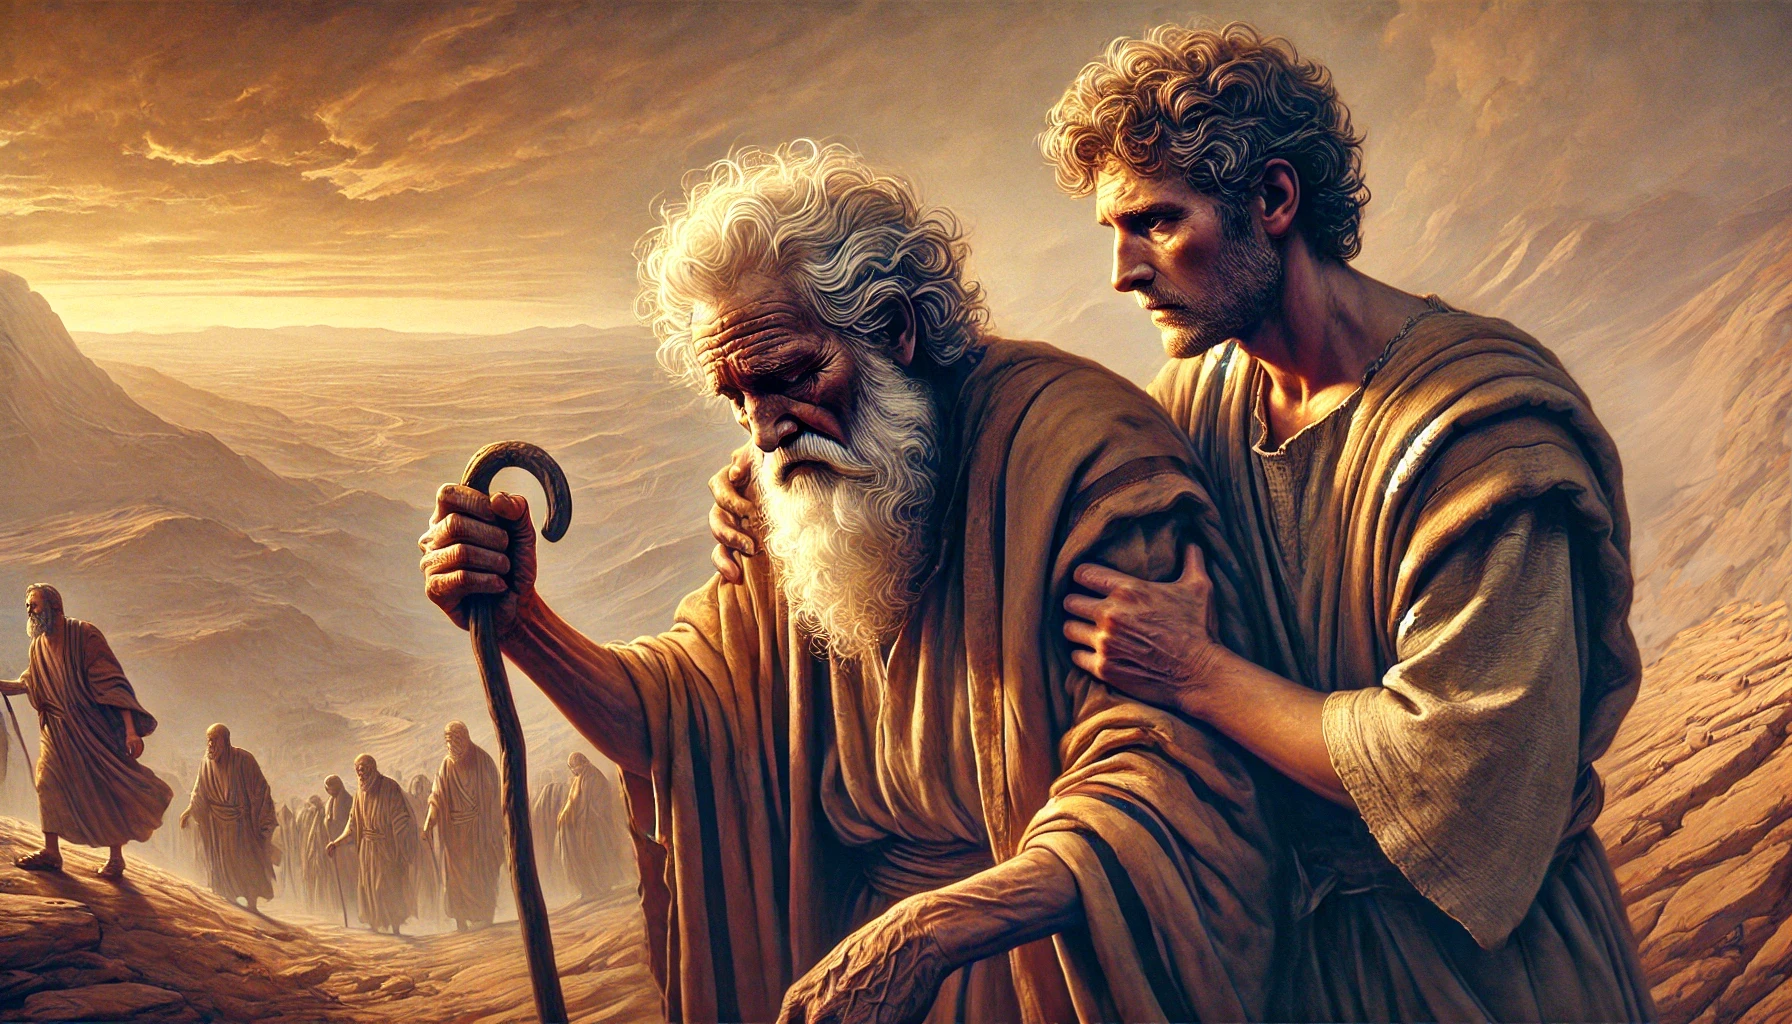
\includegraphics[width=0.7\linewidth]{graficas/deuteromonio}\\
	Moisés y Josué\\
\end{center}





\section*{Capítulo 1}


{Moisés recuerda a Israel las promesas de Jehová en Horeb } 



1:1 Estas son las palabras que habló Moisés a todo Israel a este lado del Jordán en el desierto, en el Arabá frente al Mar Rojo, entre Parán, Tofel, Labán, Hazerot y Dizahab.  
1:2 Once jornadas hay desde Horeb, camino del monte de Seir, hasta Cades-barnea.  
1:3 Y aconteció que a los cuarenta años, en el mes undécimo, el primero del mes, Moisés habló a los hijos de Israel conforme a todas las cosas que Jehová le había mandado acerca de ellos,  
1:4 después que derrotó a Sehón rey de los amorreos, el cual habitaba en Hesbón, y a Og rey de Basán que habitaba en Astarot en Edrei.  
1:5 De este lado del Jordán, en tierra de Moab, resolvió Moisés declarar esta ley, diciendo:  
1:6 Jehová nuestro Dios nos habló en Horeb, diciendo: Habéis estado bastante tiempo en este monte.  
1:7 Volveos e id al monte del amorreo y a todas sus comarcas, en el Arabá, en el monte, en los valles, en el Neguev, y junto a la costa del mar, a la tierra del cananeo, y al Líbano, hasta el gran río, el río Eufrates.  
1:8 Mirad, yo os he entregado la tierra; entrad y poseed la tierra que Jehová juró a vuestros padres Abraham, Isaac y Jacob, que les daría a ellos y a su descendencia después de ellos.  
Nombramiento de jueces   
1:9 En aquel tiempo yo os hablé diciendo: Yo solo no puedo llevaros.  
1:10 Jehová vuestro Dios os ha multiplicado, y he aquí hoy vosotros sois como las estrellas del cielo en multitud.  
1:11 ¡Jehová Dios de vuestros padres os haga mil veces más de lo que ahora sois, y os bendiga, como os ha prometido!  
1:12 ¿Cómo llevaré yo solo vuestras molestias, vuestras cargas y vuestros pleitos?  
1:13 Dadme de entre vosotros, de vuestras tribus, varones sabios y entendidos y expertos, para que yo los ponga por vuestros jefes.  
1:14 Y me respondisteis y dijisteis: Bueno es hacer lo que has dicho.  
1:15 Y tomé a los principales de vuestras tribus, varones sabios y expertos, y los puse por jefes sobre vosotros, jefes de millares, de centenas, de cincuenta y de diez, y gobernadores de vuestras tribus.  
1:16 Y entonces mandé a vuestros jueces, diciendo: Oíd entre vuestros hermanos, y juzgad justamente entre el hombre y su hermano, y el extranjero.  
1:17 No hagáis distinción de persona en el juicio; así al pequeño como al grande oiréis; no tendréis temor de ninguno, porque el juicio es de Dios; y la causa que os fuere difícil, la traeréis a mí, y yo la oiré.  
1:18 Os mandé, pues, en aquel tiempo, todo lo que habíais de hacer.  
Misión de los doce espías   
1:19 Y salidos de Horeb, anduvimos todo aquel grande y terrible desierto que habéis visto, por el camino del monte del amorreo, como Jehová nuestro Dios nos lo mandó; y llegamos hasta Cades- barnea.  
1:20 Entonces os dije: Habéis llegado al monte del amorreo, el cual Jehová nuestro Dios nos da.  
1:21 Mira, Jehová tu Dios te ha entregado la tierra; sube y toma posesión de ella, como Jehová el Dios de tus padres te ha dicho; no temas ni desmayes.  
1:22 Y vinisteis a mí todos vosotros, y dijisteis: Enviemos varones delante de nosotros que nos reconozcan la tierra, y a su regreso nos traigan razón del camino por donde hemos de subir, y de las ciudades adonde hemos de llegar.  
1:23 Y el dicho me pareció bien; y tomé doce varones de entre vosotros, un varón por cada tribu.  
1:24 Y se encaminaron, y subieron al monte, y llegaron hasta el valle de Escol, y reconocieron la tierra.  
1:25 Y tomaron en sus manos del fruto del país, y nos lo trajeron, y nos dieron cuenta, y dijeron: Es buena la tierra que Jehová nuestro Dios nos da.  
1:26 Sin embargo, no quisisteis subir, antes fuisteis rebeldes al mandato de Jehová vuestro Dios;  
1:27 y murmurasteis en vuestras tiendas, diciendo: Porque Jehová nos aborrece, nos ha sacado de tierra de Egipto, para entregarnos en manos del amorreo para destruirnos.  
1:28 ¿A dónde subiremos? Nuestros hermanos han atemorizado nuestro corazón, diciendo: Este pueblo es mayor y más alto que nosotros, las ciudades grandes y amuralladas hasta el cielo; y también vimos allí a los hijos de Anac. 
1:29 Entonces os dije: No temáis, ni tengáis miedo de ellos.  
1:30 Jehová vuestro Dios, el cual va delante de vosotros, él peleará por vosotros, conforme a todas las cosas que hizo por vosotros en Egipto delante de vuestros ojos.  
1:31 Y en el desierto has visto que Jehová tu Dios te ha traído, como trae el hombre a su hijo, por todo el camino que habéis andado, hasta llegar a este lugar.  
1:32 Y aun con esto no creísteis a Jehová vuestro Dios, 
1:33 quien iba delante de vosotros por el camino para reconoceros el lugar donde habíais de acampar, con fuego de noche para mostraros el camino por donde anduvieseis, y con nube de día.  
Dios castiga a Israel   
1:34 Y oyó Jehová la voz de vuestras palabras, y se enojó, y juró diciendo:  
1:35 No verá hombre alguno de estos, de esta mala generación, la buena tierra que juré que había de dar a vuestros padres,  
1:36 excepto Caleb hijo de Jefone; él la verá, y a él le daré la tierra que pisó, y a sus hijos; porque ha seguido fielmente a Jehová.  
1:37 También contra mí se airó Jehová por vosotros, y me dijo: Tampoco tú entrarás allá.  
1:38 Josué hijo de Nun, el cual te sirve, él entrará allá; anímale, porque él la hará heredar a Israel.  
1:39 Y vuestros niños, de los cuales dijisteis que servirían de botín, y vuestros hijos que no saben hoy lo bueno ni lo malo, ellos entrarán allá, y a ellos la daré, y ellos la heredarán.  
1:40 Pero vosotros volveos e id al desierto, camino del Mar Rojo.  
La derrota en Horma   
1:1:41 Entonces respondisteis y me dijisteis: Hemos pecado contra Jehová; nosotros subiremos y pelearemos, conforme a todo lo que Jehová nuestro Dios nos ha mandado. Y os armasteis cada uno con sus armas de guerra, y os preparasteis para subir al monte.  
1:42 Y Jehová me dijo: Diles: No subáis, ni peleéis, pues no estoy entre vosotros; para que no seáis derrotados por vuestros enemigos.  
1:43 Y os hablé, y no disteis oído; antes fuisteis rebeldes al mandato de Jehová, y persistiendo con altivez subisteis al monte.  
1:44 Pero salió a vuestro encuentro el amorreo, que habitaba en aquel monte, y os persiguieron como hacen las avispas, y os derrotaron en Seir, hasta Horma.  
1:45 Y volvisteis y llorasteis delante de Jehová, pero Jehová no escuchó vuestra voz, ni os prestó oído.  
1:46 Y estuvisteis en Cades por muchos días, los días que habéis estado allí.  
\section*{Capítulo 2}
Los años en el desierto  

2:1 Luego volvimos y salimos al desierto, camino del Mar Rojo, como Jehová me había dicho; y rodeamos el monte de Seir por mucho tiempo.  
2:2 Y Jehová me habló, diciendo:  
2:3 Bastante habéis rodeado este monte; volveos al norte.  
2:4 Y manda al pueblo, diciendo: Pasando vosotros por el territorio de vuestros hermanos los hijos de Esaú, que habitan en Seir, ellos tendrán miedo de vosotros; mas vosotros guardaos mucho.  
2:5 No os metáis con ellos, porque no os daré de su tierra ni aun lo que cubre la planta de un pie; porque yo he dado por heredad a Esaú el monte de Seir.  
2:6 Compraréis de ellos por dinero los alimentos, y comeréis; y también compraréis de ellos el agua, y beberéis;  
2:7 pues Jehová tu Dios te ha bendecido en toda obra de tus manos; él sabe que andas por este gran desierto; estos cuarenta años Jehová tu Dios ha estado contigo, y nada te ha faltado.  
2:8 Y nos alejamos del territorio de nuestros hermanos los hijos de Esaú, que habitaban en Seir, por el camino del Arabá desde Elat y Ezión-geber; y volvimos, y tomamos el camino del desierto de Moab.  
2:9 Y Jehová me dijo: No molestes a Moab, ni te empeñes con ellos en guerra, porque no te daré posesión de su tierra; porque yo he dado a Ar por heredad a los hijos de Lot.  
2:10 (Los emitas habitaron en ella antes, pueblo grande y numeroso, y alto como los hijos de Anac.  
2:11 Por gigantes eran ellos tenidos también, como los hijos de Anac; y los moabitas los llaman emitas.  
2:12 Y en Seir habitaron antes los horeos, a los cuales echaron los hijos de Esaú; y los arrojaron de su presencia, y habitaron en lugar de ellos, como hizo Israel en la tierra que les dio Jehová por posesión.)  
2:13 Levantaos ahora, y pasad el arroyo de Zered. Y pasamos el arroyo de Zered.  
2:14 Y los días que anduvimos de Cades-barnea hasta cuando pasamos el arroyo de Zered fueron treinta y ocho años; hasta que se acabó toda la generación de los hombres de guerra de en medio del campamento, como Jehová les había jurado. 
2:15 Y también la mano de Jehová vino sobre ellos para destruirlos de en medio del campamento, hasta acabarlos.  
2:16 Y aconteció que después que murieron todos los hombres de guerra de entre el pueblo,  
2:17 Jehová me habló, diciendo:  
2:18 Tú pasarás hoy el territorio de Moab, a Ar.  
2:19 Y cuando te acerques a los hijos de Amón, no los molestes, ni contiendas con ellos; porque no te daré posesión de la tierra de los hijos de Amón, pues a los hijos de Lot la he dado por heredad.  
2:20 (Por tierra de gigantes fue también ella tenida; habitaron en ella gigantes en otro tiempo, a los cuales los amonitas llamaban zomzomeos;  
2:21 pueblo grande y numeroso, y alto, como los hijos de Anac; a los cuales Jehová destruyó delante de los amonitas. Estos sucedieron a aquéllos, y habitaron en su lugar,  
2:22 como hizo Jehová con los hijos de Esaú que habitaban en Seir, delante de los cuales destruyó a los horeos; y ellos sucedieron a éstos, y habitaron en su lugar hasta hoy.  
2:23 Y a los aveos que habitaban en aldeas hasta Gaza, los caftoreos que salieron de Caftor los destruyeron, y habitaron en su lugar.)  
2:24 Levantaos, salid, y pasad el arroyo de Arnón; he aquí he entregado en tu mano a Sehón rey de Hesbón, amorreo, y a su tierra; comienza a tomar posesión de ella, y entra en guerra con él.  
2:25 Hoy comenzaré a poner tu temor y tu espanto sobre los pueblos debajo de todo el cielo, los cuales oirán tu fama, y temblarán y se angustiarán delante de ti.  
Israel derrota a Sehón   
2:26 Y envié mensajeros desde el desierto de Cademot a Sehón rey de Hesbón con palabras de paz, diciendo:  
2:27 Pasaré por tu tierra por el camino; por el camino iré, sin apartarme ni a diestra ni a siniestra.  
2:28 La comida me venderás por dinero, y comeré; el agua también me darás por dinero, y beberé; solamente pasaré a pie,  
2:29 como lo hicieron conmigo los hijos de Esaú que habitaban en Seir, y los moabitas que habitaban en Ar; hasta que cruce el Jordán a la tierra que nos da Jehová nuestro Dios.  
2:30 Mas Sehón rey de Hesbón no quiso que pasásemos por el territorio suyo; porque Jehová tu Dios había endurecido su espíritu, y obstinado su corazón para entregarlo en tu mano, como hasta hoy.  
2:31 Y me dijo Jehová: He aquí yo he comenzado a entregar delante de ti a Sehón y a su tierra; comienza a tomar posesión de ella para que la heredes.  
2:32 Y nos salió Sehón al encuentro, él y todo su pueblo, para pelear en Jahaza.  
2:33 Mas Jehová nuestro Dios lo entregó delante de nosotros; y lo derrotamos a él y a sus hijos, y a todo su pueblo.  
2:34 Tomamos entonces todas sus ciudades, y destruimos todas las ciudades, hombres, mujeres y niños; no dejamos ninguno.  
2:35 Solamente tomamos para nosotros los ganados, y los despojos de las ciudades que habíamos tomado.  
2:36 Desde Aroer, que está junto a la ribera del arroyo de Arnón, y la ciudad que está en el valle, hasta Galaad, no hubo ciudad que escapase de nosotros; todas las entregó Jehová nuestro Dios en nuestro poder.  
2:37 Solamente a la tierra de los hijos de Amón no llegamos; ni a todo lo que está a la orilla del arroyo de Jaboc ni a las ciudades del monte, ni a lugar alguno que Jehová nuestro Dios había prohibido.  
\section*{Capítulo 3}
Israel derrota a Og rey de Basán  

3:1 Volvimos, pues, y subimos camino de Basán, y nos salió al encuentro Og rey de Basán para pelear, él y todo su pueblo, en Edrei.  
3:2 Y me dijo Jehová: No tengas temor de él, porque en tu mano he entregdo a él y a todo su pueblo, con su tierra; y harás con él como hiciste con Sehón rey amorreo, que habitaba en Hesbón.  
3:3 Y Jehová nuestro Dios entregó también en nuestra mano a Og rey de Basán, y a todo su pueblo, al cual derrotamos hasta acabar con todos.  
3:4 Y tomamos entonces todas sus ciudades; no quedó ciudad que no les tomásemos; sesenta ciudades, toda la tierra de Argob, del reino de Og en Basán.  
3:5 Todas estas eran ciudades fortificadas con muros altos, con puertas y barras, sin contar otras muchas ciudades sin muro.  
3:6 Y las destruimos, como hicimos a Sehón rey de Hesbón, matando en toda ciudad a hombres, mujeres y niños.  
3:7 Y tomamos para nosotros todo el ganado, y los despojos de las ciudades.  
3:8 También tomamos en aquel tiempo la tierra desde el arroyo de Arnón hasta el monte de Hermón, de manos de los dos reyes amorreos que estaban a este lado del Jordán.  
3:9 (Los sidonios llaman a Hermón, Sirión; y los amorreos, Senir.)  
3:10 Todas las ciudades de la llanura, y todo Galaad, y todo Basán hasta Salca y Edrei, ciudades del reino de Og en Basán.  
3:11 Porque únicamente Og rey de Basán había quedado del resto de los gigantes. Su cama, una cama de hierro, ¿no está en Rabá de los hijos de Amón? La longitud de ella es de nueve codos, y su anchura de cuatro codos, según el codo de un hombre.  
Rubén, Gad y la media tribu de Manasés se establecen al oriente del Jordán  

3:12 Y esta tierra que heredamos en aquel tiempo, desde Aroer, que está junto al arroyo de Arnón, y la mitad del monte de Galaad con sus ciudades, la di a los rubenitas y a los gaditas;  
3:13 y el resto de Galaad, y todo Basán, del reino de Og, toda la tierra de Argob, que se llamaba la tierra de los gigantes, lo di a la media tribu de Manasés.  
3:14 Jair hijo de Manasés tomó toda la tierra de Argob hasta el límite con Gesur y Maaca, y la llamó por su nombre, Basán- havot-jair, hasta hoy.  
3:15 Y Galaad se lo di a Maquir.  
3:16 Y a los rubenitas y gaditas les di de Galaad hasta el arroyo de Arnón, teniendo por límite el medio del valle, hasta el arroyo de Jaboc, el cual es límite de los hijos de Amón;  
3:17 también el Arabá, con el Jordán como límite desde Cineret hasta el mar del Arabá, el Mar Salado, al pie de las laderas del Pisga al oriente.  
3:18 Y os mandé entonces, diciendo: Jehová vuestro Dios os ha dado esta tierra por heredad; pero iréis armados todos los valientes delante de vuestros hermanos los hijos de Israel.  
3:19 Solamente vuestras mujeres, vuestros hijos y vuestros ganados (yo sé que tenéis mucho ganado), quedarán en las ciudades que os he dado,  
3:20 hasta que Jehová dé reposo a vuestros hermanos, así como a vosotros, y hereden ellos también la tierra que Jehová vuestro Dios les da al otro lado del Jordán; entonces os volveréis cada uno a la heredad que yo os he dado.  
3:21 Ordené también a Josué en aquel tiempo, diciendo: Tus ojos vieron todo lo que Jehová vuestro Dios ha hecho a aquellos dos reyes; así hará Jehová a todos los reinos a los cuales pasarás tú.  
3:22 No los temáis; porque Jehová vuestro Dios, él es el que pelea por vosotros.  
No se le permite a Moisés entrar a Canaán  
3:23 Y oré a Jehová en aquel tiempo, diciendo:  
3:24 Señor Jehová, tú has comenzado a mostrar a tu siervo tu grandeza, y tu mano poderosa; porque ¿qué dios hay en el cielo ni en la tierra que haga obras y proezas como las tuyas?  
3:25 Pase yo, te ruego, y vea aquella tierra buena que está más allá del Jordán, aquel buen monte, y el Líbano.  
3:26 Pero Jehová se había enojado contra mí a causa de vosotros, por lo cual no me escuchó; y me dijo Jehová: Basta, no me hables más de este asunto.  
3:27 Sube a la cumbre del Pisga y alza tus ojos al oeste, y al norte, y al sur, y al este, y mira con tus propios ojos; porque no pasarás el Jordán.  
3:28 Y manda a Josué, y anímalo, y fortalécelo; porque él ha de pasar delante de este pueblo, y él les hará heredar la tierra que verás.  
3:29 Y paramos en el valle delante de Bet-peor.  
\section*{Capítulo 4 }
Moisés exhorta a la obediencia  

4:1 Ahora, pues, oh Israel, oye los estatutos y decretos que yo os enseño, para que los ejecutéis, y viváis, y entréis y poseáis la tierra que Jehová el Dios de vuestros padres os da.  
4:2 No añadiréis a la palabra que yo os mando, ni disminuiréis de ella, para que guardéis los mandamientos de Jehová vuestro Dios que yo os ordene.  
4:3 Vuestros ojos vieron lo que hizo Jehová con motivo de Baal- peor; que a todo hombre que fue en pos de Baal-peor destruyó Jehová tu Dios de en medio de ti.  
4:4 Mas vosotros que seguisteis a Jehová vuestro Dios, todos estáis vivos hoy.  
4:5 Mirad, yo os he enseñado estatutos y decretos, como Jehová mi Dios me mandó, para que hagáis así en medio de la tierra en la cual entráis para tomar posesión de ella.  
4:6 Guardadlos, pues, y ponedlos por obra; porque esta es vuestra sabiduría y vuestra inteligencia ante los ojos de los pueblos, los cuales oirán todos estos estatutos, y dirán: Ciertamente pueblo sabio y entendido, nación grande es esta.  
4:7 Porque ¿qué nación grande hay que tenga dioses tan cercanos a ellos como lo está Jehová nuestro Dios en todo cuanto le pedimos?  
4:8 Y ¿qué nación grande hay que tenga estatutos y juicios justos como es toda esta ley que yo pongo hoy delante de vosotros?  
La experiencia de Israel en Horeb  
4:9 Por tanto, guárdate, y guarda tu alma con diligencia, para que no te olvides de las cosas que tus ojos han visto, ni se aparten de tu corazón todos los días de tu vida; antes bien, las enseñarás a tus hijos, y a los hijos de tus hijos.  
4:10 El día que estuviste delante de Jehová tu Dios en Horeb, cuando Jehová me dijo: Reúneme el pueblo, para que yo les haga oír mis palabras, las cuales aprenderán, para temerme todos los días que vivieren sobre la tierra, y las enseñarán a sus hijos;  
4:11 y os acercasteis y os pusisteis al pie del monte; y el monte ardía en fuego hasta en medio de los cielos con tinieblas, nube y oscuridad;  
4:12 y habló Jehová con vosotros de en medio del fuego; oísteis la voz de sus palabras, mas a excepción de oír la voz, ninguna figura visteis.  
4:13 Y él os anunció su pacto, el cual os mandó poner por obra; los diez mandamientos, y los escribió en dos tablas de piedra. 
4:14 A mí también me mandó Jehová en aquel tiempo que os enseñase los estatutos y juicios, para que los pusieseis por obra en la tierra a la cual pasáis a tomar posesión de ella.  
Advertencia contra la idolatría  
4:15 Guardad, pues, mucho vuestras almas; pues ninguna figura visteis el día que Jehová habló con vosotros de en medio del fuego;  
4:16 para que no os corrompáis y hagáis para vosotros escultura, imagen de figura alguna, efigie de varón o hembra,  
4:17 figura de animal alguno que está en la tierra, figura de ave alguna alada que vuele por el aire,  
4:18 figura de ningún animal que se arrastre sobre la tierra, figura de pez alguno que haya en el agua debajo de la tierra.  
4:19 No sea que alces tus ojos al cielo, y viendo el sol y la luna y las estrellas, y todo el ejército del cielo, seas impulsado, y te inclines a ellos y les sirvas; porque Jehová tu Dios los ha concedido a todos los pueblos debajo de todos los cielos.  
4:20 Pero a vosotros Jehová os tomó, y os ha sacado del horno de hierro, de Egipto, para que seáis el pueblo de su heredad como en este día.  
4:21 Y Jehová se enojó contra mí por causa de vosotros, y juró que yo no pasaría el Jordán, ni entraría en la buena tierra que Jehová tu Dios te da por heredad.  
4:22 Así que yo voy a morir en esta tierra, y no pasaré el Jordán; mas vosotros pasaréis, y poseeréis aquella buena tierra.  
4:23 Guardaos, no os olvidéis del pacto de Jehová vuestro Dios, que él estableció con vosotros, y no os hagáis escultura o imagen de ninguna cosa que Jehová tu Dios te ha prohibido.  
4:24 Porque Jehová tu Dios es fuego consumidor, Dios celoso.  
4:25 Cuando hayáis engendrado hijos y nietos, y hayáis envejecido en la tierra, si os corrompiereis e hiciereis escultura o imagen de cualquier cosa, e hiciereis lo malo ante los ojos de Jehová vuestro Dios, para enojarlo;  
4:26 yo pongo hoy por testigos al cielo y a la tierra, que pronto pereceréis totalmente de la tierra hacia la cual pasáis el Jordán para tomar posesión de ella; no estaréis en ella largos días sin que seáis destruidos.  
4:27 Y Jehová os esparcirá entre los pueblos, y quedaréis pocos en número entre las naciones a las cuales os llevará Jehová.  
4:28 Y serviréis allí a dioses hechos de manos de hombres, de madera y piedra, que no ven, ni oyen, ni comen, ni huelen.  
4:29 Mas si desde allí buscares a Jehová tu Dios, lo hallarás, si lo buscares de todo tu corazón y de toda tu alma.  
4:30 Cuando estuvieres en angustia, y te alcanzaren todas estas cosas, si en los postreros días te volvieres a Jehová tu Dios, y oyeres su voz;  
4:31 porque Dios misericordioso es Jehová tu Dios; no te dejará, ni te destruirá, ni se olvidará del pacto que les juró a tus padres.  
4:32 Porque pregunta ahora si en los tiempos pasados que han sido antes de ti, desde el día que creó Dios al hombre sobre la tierra, si desde un extremo del cielo al otro se ha hecho cosa semejante a esta gran cosa, o se haya oído otra como ella.  
4:33 ¿Ha oído pueblo alguno la voz de Dios, hablando de en medio del fuego, como tú la has oído, sin perecer?  
4:34 ¿O ha intentado Dios venir a tomar para sí una nación de en medio de otra nación, con pruebas, con señales, con milagros y con guerra, y mano poderosa y brazo extendido, y hechos aterradores como todo lo que hizo con vosotros Jehová vuestro Dios en Egipto ante tus ojos?  
4:35 A ti te fue mostrado, para que supieses que Jehová es Dios, y no hay otro fuera de él.  
4:36 Desde los cielos te hizo oír su voz, para enseñarte; y sobre la tierra te mostró su gran fuego, y has oído sus palabras de en medio del fuego.  
4:37 Y por cuanto él amó a tus padres, escogió a su descendencia después de ellos, y te sacó de Egipto con su presencia y con su gran poder,  
4:38 para echar de delante de tu presencia naciones grandes y más fuertes que tú, y para introducirte y darte su tierra por heredad, como hoy.  
4:39 Aprende pues, hoy, y reflexiona en tu corazón que Jehová es Dios arriba en el cielo y abajo en la tierra, y no hay otro.  
4:40 Y guarda sus estatutos y sus mandamientos, los cuales yo te mando hoy, para que te vaya bien a ti y a tus hijos después de ti, y prolongues tus días sobre la tierra que Jehová tu Dios te da para siempre.  
Las ciudades de refugio al oriente del Jordán  
4:41 Entonces apartó Moisés tres ciudades a este lado del Jordán al nacimiento del sol,  
4:42 para que huyese allí el homicida que matase a su prójimo sin intención, sin haber tenido enemistad con él nunca antes; y que huyendo a una de estas ciudades salvase su vida:  
4:43 Beser en el desierto, en tierra de la llanura, para los rubenitas; Ramot en Galaad para los gaditas, y Golán en Basán para los de Manasés.  
Moisés recapitula la promulgación de la ley  
4:44 Esta, pues, es la ley que Moisés puso delante de los hijos de Israel.  
4:45 Estos son los testimonios, los estatutos y los decretos que habló Moisés a los hijos de Israel cuando salieron de Egipto;  
4:46 a este lado del Jordán, en el valle delante de Bet-peor, en la tierra de Sehón rey de los amorreos que habitaba en Hesbón, al cual derrotó Moisés con los hijos de Israel, cuando salieron de Egipto;  
4:47 y poseyeron su tierra, y la tierra de Og rey de Basán; dos reyes de los amorreos que estaban de este lado del Jordán, al oriente. 
4:48 Desde Aroer, que está junto a la ribera del arroyo de Arnón, hasta el monte de Sion, que es Hermón; 
4:49 y todo el Arabá de este lado del Jordán, al oriente, hasta el mar del Arabá, al pie de las laderas del Pisga.  
\section*{Capítulo 5 }
Los Diez Mandamientos   

5:1 Llamó Moisés a todo Israel y les dijo: Oye, Israel, los estatutos y decretos que yo pronuncio hoy en vuestros oídos; aprendedlos, y guardadlos, para ponerlos por obra.  
5:2 Jehová nuestro Dios hizo pacto con nosotros en Horeb.  
5:3 No con nuestros padres hizo Jehová este pacto, sino con nosotros todos los que estamos aquí hoy vivos.  
5:4 Cara a cara habló Jehová con vosotros en el monte de en medio del fuego.  
5:5 Yo estaba entonces entre Jehová y vosotros, para declararos la palabra de Jehová; porque vosotros tuvisteis temor del fuego, y no subisteis al monte. Dijo:  
5:6 Yo soy Jehová tu Dios, que te saqué de tierra de Egipto, de casa de servidumbre.  
5:7 No tendrás dioses ajenos delante de mí.  
5:8 No harás para ti escultura, ni imagen alguna de cosa que está arriba en los cielos, ni abajo en la tierra, ni en las aguas debajo de la tierra.  
5:9 No te inclinarás a ellas ni las servirás; porque yo soy Jehová tu Dios, fuerte, celoso, que visito la maldad de los padres sobre los hijos hasta la tercera y cuarta generación de los que me aborrecen,  
5:10 y que hago misericordia a millares, a los que me aman y guardan mis mandamientos.  
5:11 No tomarás el nombre de Jehová tu Dios en vano; porque Jehová no dará por inocente al que tome su nombre en vano.  
5:12 Guardarás el día de reposo para santificarlo, como Jehová tu Dios te ha mandado. 
5:13 Seis días trabajarás, y harás toda tu obra;  
5:14 mas el séptimo día es reposo a Jehová tu Dios; ninguna obra harás tú, ni tu hijo, ni tu hija, ni tu siervo, ni tu sierva, ni tu buey, ni tu asno, ni ningún animal tuyo, ni el extranjero que está dentro de tus puertas, para que descanse tu siervo y tu sierva como tú.  
5:15 Acuérdate que fuiste siervo en tierra de Egipto, y que Jehová tu Dios te sacó de allá con mano fuerte y brazo extendido; por lo cual Jehová tu Dios te ha mandado que guardes el día de reposo.  
5:16 Honra a tu padre y a tu madre, como Jehová tu Dios te ha mandado, para que sean prolongados tus días, y para que te vaya bien sobre la tierra que Jehová tu Dios te da.  
5:17 No matarás. 
5:18 No cometerás adulterio.  
5:19 No hurtarás. 
5:20 No dirás falso testimonio contra tu prójimo.  
5:21 No codiciarás la mujer de tu prójimo, ni desearás la casa de tu prójimo, ni su tierra, ni su siervo, ni su sierva, ni su buey, ni su asno, ni cosa alguna de tu prójimo.  
El terror del pueblo   
5:22 Estas palabras habló Jehová a toda vuestra congregación en el monte, de en medio del fuego, de la nube y de la oscuridad, a gran voz; y no añadió más. Y las escribió en dos tablas de piedra, las cuales me dio a mí.  
5:23 Y aconteció que cuando vosotros oísteis la voz de en medio de las tinieblas, y visteis al monte que ardía en fuego, vinisteis a mí, todos los príncipes de vuestras tribus, y vuestros ancianos,  
5:24 y dijisteis: He aquí Jehová nuestro Dios nos ha mostrado su gloria y su grandeza, y hemos oído su voz de en medio del fuego; hoy hemos visto que Jehová habla al hombre, y éste aún vive.  
5:25 Ahora, pues, ¿por qué vamos a morir? Porque este gran fuego nos consumirá; si oyéremos otra vez la voz de Jehová nuestro Dios, moriremos.  
5:26 Porque ¿qué es el hombre, para que oiga la voz del Dios viviente que habla de en medio del fuego, como nosotros la oímos, y aún viva?  
5:27 Acércate tú, y oye todas las cosas que dijere Jehová nuestro Dios; y tú nos dirás todo lo que Jehová nuestro Dios te dijere, y nosotros oiremos y haremos.  
5:28 Y oyó Jehová la voz de vuestras palabras cuando me hablabais, y me dijo Jehová: He oído la voz de las palabras de este pueblo, que ellos te han hablado; bien está todo lo que han dicho.  
5:29 ¡Quién diera que tuviesen tal corazón, que me temiesen y guardasen todos los días todos mis mandamientos, para que a ellos y a sus hijos les fuese bien para siempre!  
5:30 Ve y diles: Volveos a vuestras tiendas.  
5:31 Y tú quédate aquí conmigo, y te diré todos los mandamientos y estatutos y decretos que les enseñarás, a fin de que los pongan ahora por obra en la tierra que yo les doy por posesión.  
5:32 Mirad, pues, que hagáis como Jehová vuestro Dios os ha mandado; no os apartéis a diestra ni a siniestra.  
5:33 Andad en todo el camino que Jehová vuestro Dios os ha mandado, para que viváis y os vaya bien, y tengáis largos días en la tierra que habéis de poseer.  
\section*{Capítulo 6 }
El gran mandamiento  

6:1 Estos, pues, son los mandamientos, estatutos y decretos que Jehová vuestro Dios mandó que os enseñase, para que los pongáis por obra en la tierra a la cual pasáis vosotros para tomarla;  
6:2 para que temas a Jehová tu Dios, guardando todos sus estatutos y sus mandamientos que yo te mando, tú, tu hijo, y el hijo de tu hijo, todos los días de tu vida, para que tus días sean prolongados.  
6:3 Oye, pues, oh Israel, y cuida de ponerlos por obra, para que te vaya bien en la tierra que fluye leche y miel, y os multipliquéis, como te ha dicho Jehová el Dios de tus padres.  
6:4 Oye, Israel: Jehová nuestro Dios, Jehová uno es.  
6:5 Y amarás a Jehová tu Dios de todo tu corazón, y de toda tu alma, y con todas tus fuerzas.  
6:6 Y estas palabras que yo te mando hoy, estarán sobre tu corazón;  
6:7 y las repetirás a tus hijos, y hablarás de ellas estando en tu casa, y andando por el camino, y al acostarte, y cuando te levantes.  
6:8 Y las atarás como una señal en tu mano, y estarán como frontales entre tus ojos;  
6:9 y las escribirás en los postes de tu casa, y en tus puertas.  
Exhortaciones a la obediencia  
6:10 Cuando Jehová tu Dios te haya introducido en la tierra que juró a tus padres Abraham, Isaac y Jacob que te daría, en ciudades grandes y buenas que tú no edificaste,  
6:11 y casas llenas de todo bien, que tú no llenaste, y cisternas cavadas que tú no cavaste, viñas y olivares que no plantaste, y luego que comas y te sacies,  
6:12 cuídate de no olvidarte de Jehová, que te sacó de la tierra de Egipto, de casa de servidumbre.  
6:13 A Jehová tu Dios temerás, y a él solo servirás, y por su nombre jurarás.  
6:14 No andaréis en pos de dioses ajenos, de los dioses de los pueblos que están en vuestros contornos;  
6:15 porque el Dios celoso, Jehová tu Dios, en medio de ti está; para que no se inflame el furor de Jehová tu Dios contra ti, y te destruya de sobre la tierra.  
6:16 No tentaréis a Jehová vuestro Dios, como lo tentasteis en Masah.  
6:17 Guardad cuidadosamente los mandamientos de Jehová vuestro Dios, y sus testimonios y sus estatutos que te ha mandado.  
6:18 Y haz lo recto y bueno ante los ojos de Jehová, para que te vaya bien, y entres y poseas la buena tierra que Jehová juró a tus padres;  
6:19 para que él arroje a tus enemigos de delante de ti, como Jehová ha dicho.  
6:20 Mañana cuando te preguntare tu hijo, diciendo: ¿Qué significan los testimonios y estatutos y decretos que Jehová nuestro Dios os mandó?  
6:21 entonces dirás a tu hijo: Nosotros éramos siervos de Faraón en Egipto, y Jehová nos sacó de Egipto con mano poderosa.  
6:22 Jehová hizo señales y milagros grandes y terribles en Egipto, sobre Faraón y sobre toda su casa, delante de nuestros ojos;  
6:23 y nos sacó de allá, para traernos y darnos la tierra que juró a nuestros padres.  
6:24 Y nos mandó Jehová que cumplamos todos estos estatutos, y que temamos a Jehová nuestro Dios, para que nos vaya bien todos los días, y para que nos conserve la vida, como hasta hoy.  
6:25 Y tendremos justicia cuando cuidemos de poner por obra todos estos mandamientos delante de Jehová nuestro Dios, como él nos ha mandado.  
\section*{Capítulo 7 }
Advertencias contra la idolatría de Canaán   

7:1 Cuando Jehová tu Dios te haya introducido en la tierra en la cual entrarás para tomarla, y haya echado de delante de ti a muchas naciones, al heteo, al gergeseo, al amorreo, al cananeo, al ferezeo, al heveo y al jebuseo, siete naciones mayores y más poderosas que tú,  
7:2 y Jehová tu Dios las haya entregado delante de ti, y las hayas derrotado, las destruirás del todo; no harás con ellas alianza, ni tendrás de ellas misericordia.  
7:3 Y no emparentarás con ellas; no darás tu hija a su hijo, ni tomarás a su hija para tu hijo.  
7:4 Porque desviará a tu hijo de en pos de mí, y servirán a dioses ajenos; y el furor de Jehová se encenderá sobre vosotros, y te destruirá pronto.  
7:5 Mas así habéis de hacer con ellos: sus altares destruiréis, y quebraréis sus estatuas, y destruiréis sus imágenes de Asera, y quemaréis sus esculturas en el fuego.  
Un pueblo santo para Jehová  
7:6 Porque tú eres pueblo santo para Jehová tu Dios; Jehová tu Dios te ha escogido para serle un pueblo especial, más que todos los pueblos que están sobre la tierra.  
7:7 No por ser vosotros más que todos los pueblos os ha querido Jehová y os ha escogido, pues vosotros erais el más insignificante de todos los pueblos;  
7:8 sino por cuanto Jehová os amó, y quiso guardar el juramento que juró a vuestros padres, os ha sacado Jehová con mano poderosa, y os ha rescatado de servidumbre, de la mano de Faraón rey de Egipto.  
7:9 Conoce, pues, que Jehová tu Dios es Dios, Dios fiel, que guarda el pacto y la misericordia a los que le aman y guardan sus mandamientos, hasta mil generaciones;  
7:10 y que da el pago en persona al que le aborrece, destruyéndolo; y no se demora con el que le odia, en persona le dará el pago.  
7:11 Guarda, por tanto, los mandamientos, estatutos y decretos que yo te mando hoy que cumplas.  
Bendiciones de la obediencia   
7:12 Y por haber oído estos decretos y haberlos guardado y puesto por obra, Jehová tu Dios guardará contigo el pacto y la misericordia que juró a tus padres.  
7:13 Y te amará, te bendecirá y te multiplicará, y bendecirá el fruto de tu vientre y el fruto de tu tierra, tu grano, tu mosto, tu aceite, la cría de tus vacas, y los rebaños de tus ovejas, en la tierra que juró a tus padres que te daría.  
7:14 Bendito serás más que todos los pueblos; no habrá en ti varón ni hembra estéril, ni en tus ganados.  
7:15 Y quitará Jehová de ti toda enfermedad; y todas las malas plagas de Egipto, que tú conoces, no las pondrá sobre ti, antes las pondrá sobre todos los que te aborrecieren.  
7:16 Y consumirás a todos los pueblos que te da Jehová tu Dios; no los perdonará tu ojo, ni servirás a sus dioses, porque te será tropiezo.  
7:17 Si dijeres en tu corazón: Estas naciones son mucho más numerosas que yo; ¿cómo las podré exterminar?  
7:18 no tengas temor de ellas; acuérdate bien de lo que hizo Jehová tu Dios con Faraón y con todo Egipto;  
7:19 de las grandes pruebas que vieron tus ojos, y de las señales y milagros, y de la mano poderosa y el brazo extendido con que Jehová tu Dios te sacó; así hará Jehová tu Dios con todos los pueblos de cuya presencia tú temieres.  
7:20 También enviará Jehová tu Dios avispas sobre ellos, hasta que perezcan los que quedaren y los que se hubieren escondido de delante de ti.  
7:21 No desmayes delante de ellos, porque Jehová tu Dios está en medio de ti, Dios grande y temible.  
7:22 Y Jehová tu Dios echará a estas naciones de delante de ti poco a poco; no podrás acabar con ellas en seguida, para que las fieras del campo no se aumenten contra ti.  
7:23 Mas Jehová tu Dios las entregará delante de ti, y él las quebrantará con grande destrozo, hasta que sean destruidas.  
7:24 El entregará sus reyes en tu mano, y tú destruirás el nombre de ellos de debajo del cielo; nadie te hará frente hasta que los destruyas.  
7:25 Las esculturas de sus dioses quemarás en el fuego; no codiciarás plata ni oro de ellas para tomarlo para ti, para que no tropieces en ello, pues es abominación a Jehová tu Dios;  
7:26 y no traerás cosa abominable a tu casa, para que no seas anatema; del todo la aborrecerás y la abominarás, porque es anatema.  
\section*{Capítulo 8 }
La buena tierra que han de poseer  

8:1 Cuidaréis de poner por obra todo mandamiento que yo os ordeno hoy, para que viváis, y seáis multiplicados, y entréis y poseáis la tierra que Jehová prometió con juramento a vuestros padres.  
8:2 Y te acordarás de todo el camino por donde te ha traído Jehová tu Dios estos cuarenta años en el desierto, para afligirte, para probarte, para saber lo que había en tu corazón, si habías de guardar o no sus mandamientos.  
8:3 Y te afligió, y te hizo tener hambre, y te sustentó con maná, comida que no conocías tú, ni tus padres la habían conocido, para hacerte saber que no sólo de pan vivirá el hombre, mas de todo lo que sale de la boca de Jehová vivirá el hombre.  
8:4 Tu vestido nunca se envejeció sobre ti, ni el pie se te ha hinchado en estos cuarenta años.  
8:5 Reconoce asimismo en tu corazón, que como castiga el hombre a su hijo, así Jehová tu Dios te castiga.  
8:6 Guardarás, pues, los mandamientos de Jehová tu Dios, andando en sus caminos, y temiéndole.  
8:7 Porque Jehová tu Dios te introduce en la buena tierra, tierra de arroyos, de aguas, de fuentes y de manantiales, que brotan en vegas y montes;  
8:8 tierra de trigo y cebada, de vides, higueras y granados; tierra de olivos, de aceite y de miel;  
8:9 tierra en la cual no comerás el pan con escasez, ni te faltará nada en ella; tierra cuyas piedras son hierro, y de cuyos montes sacarás cobre.  
8:10 Y comerás y te saciarás, y bendecirás a Jehová tu Dios por la buena tierra que te habrá dado.  
Amonestación de no olvidar a Dios  
8:11 Cuídate de no olvidarte de Jehová tu Dios, para cumplir sus mandamientos, sus decretos y sus estatutos que yo te ordeno hoy;  
8:12 no suceda que comas y te sacies, y edifiques buenas casas en que habites,  
8:13 y tus vacas y tus ovejas se aumenten, y la plata y el oro se te multipliquen, y todo lo que tuvieres se aumente;  
8:14 y se enorgullezca tu corazón, y te olvides de Jehová tu Dios, que te sacó de tierra de Egipto, de casa de servidumbre;  
8:15 que te hizo caminar por un desierto grande y espantoso, lleno de serpientes ardientes, y de escorpiones, y de sed, donde no había agua, y él te sacó agua de la roca del pedernal;  
8:16 que te sustentó con maná en el desierto, comida que tus padres no habían conocido, afligiéndote y probándote, para a la postre hacerte bien;  
8:17 y digas en tu corazón: Mi poder y la fuerza de mi mano me han traído esta riqueza.  
8:18 Sino acuérdate de Jehová tu Dios, porque él te da el poder para hacer las riquezas, a fin de confirmar su pacto que juró a tus padres, como en este día.  
8:19 Mas si llegares a olvidarte de Jehová tu Dios y anduvieres en pos de dioses ajenos, y les sirvieres y a ellos te inclinares, yo lo afirmo hoy contra vosotros, que de cierto pereceréis.  
8:20 Como las naciones que Jehová destruirá delante de vosotros, así pereceréis, por cuanto no habréis atendido a la voz de Jehová vuestro Dios.  
\section*{Capítulo 9}
Dios destruirá a las naciones de Canaán  

9:1 Oye, Israel: tú vas hoy a pasar el Jordán, para entrar a desposeer a naciones más numerosas y más poderosas que tú, ciudades grandes y amuralladas hasta el cielo;  
9:2 un pueblo grande y alto, hijos de los anaceos, de los cuales tienes tú conocimiento, y has oído decir: ¿Quién se sostendrá delante de los hijos de Anac?  
9:3 Entiende, pues, hoy, que es Jehová tu Dios el que pasa delante de ti como fuego consumidor, que los destruirá y humillará delante de ti; y tú los echarás, y los destruirás en seguida, como Jehová te ha dicho.  
9:4 No pienses en tu corazón cuando Jehová tu Dios los haya echado de delante de ti, diciendo: Por mi justicia me ha traído Jehová a poseer esta tierra; pues por la impiedad de estas naciones Jehová las arroja de delante de ti.  
9:5 No por tu justicia, ni por la rectitud de tu corazón entras a poseer la tierra de ellos, sino por la impiedad de estas naciones Jehová tu Dios las arroja de delante de ti, y para confirmar la palabra que Jehová juró a tus padres Abraham, Isaac y Jacob.  
La rebelión de Israel en Horeb   
9:6 Por tanto, sabe que no es por tu justicia que Jehová tu Dios te da esta buena tierra para tomarla; porque pueblo duro de cerviz eres tú. 
9:7 Acuérdate, no olvides que has provocado la ira de Jehová tu Dios en el desierto; desde el día que saliste de la tierra de Egipto, hasta que entrasteis en este lugar, habéis sido rebeldes a Jehová.  
9:8 En Horeb provocasteis a ira a Jehová, y se enojó Jehová contra vosotros para destruiros.  
9:9 Cuando yo subí al monte para recibir las tablas de piedra, las tablas del pacto que Jehová hizo con vosotros, estuve entonces en el monte cuarenta días y cuarenta noches, sin comer pan ni beber agua;  
9:10 y me dio Jehová las dos tablas de piedra escritas con el dedo de Dios; y en ellas estaba escrito según todas las palabras que os habló Jehová en el monte, de en medio del fuego, el día de la asamblea.  
9:11 Sucedió al fin de los cuarenta días y cuarenta noches, que Jehová me dio las dos tablas de piedra, las tablas del pacto.  
9:12 Y me dijo Jehová: Levántate, desciende pronto de aquí, porque tu pueblo que sacaste de Egipto se ha corrompido; pronto se han apartado del camino que yo les mandé; se han hecho una imagen de fundición.  
9:13 Y me habló Jehová, diciendo: He observado a ese pueblo, y he aquí que es pueblo duro de cerviz.  
9:14 Déjame que los destruya, y borre su nombre de debajo del cielo, y yo te pondré sobre una nación fuerte y mucho más numerosa que ellos.  
9:15 Y volví y descendí del monte, el cual ardía en fuego, con las tablas del pacto en mis dos manos.  
9:16 Y miré, y he aquí habíais pecado contra Jehová vuestro Dios; os habíais hecho un becerro de fundición, apartándoos pronto del camino que Jehová os había mandado.  
9:17 Entonces tomé las dos tablas y las arrojé de mis dos manos, y las quebré delante de vuestros ojos.  
9:18 Y me postré delante de Jehová como antes, cuarenta días y cuarenta noches; no comí pan ni bebí agua, a causa de todo vuestro pecado que habíais cometido haciendo el mal ante los ojos de Jehová para enojarlo. 
9:19 Porque temí a causa del furor y de la ira con que Jehová estaba enojado contra vosotros para destruiros. Pero Jehová me escuchó aun esta vez.  
9:20 Contra Aarón también se enojó Jehová en gran manera para destruirlo; y también oré por Aarón en aquel entonces.  
9:21 Y tomé el objeto de vuestro pecado, el becerro que habíais hecho, y lo quemé en el fuego, y lo desmenucé moliéndolo muy bien, hasta que fue reducido a polvo; y eché el polvo de él en el arroyo que descendía del monte.  
9:22 También en Tabera, en Masah y en Kibrot-hataava  provocasteis a ira a Jehová.  
9:23 Y cuando Jehová os envió desde Cades-barnea, diciendo: Subid y poseed la tierra que yo os he dado, también fuisteis rebeldes al mandato de Jehová vuestro Dios, y no le creísteis, ni obedecisteis a su voz.  
9:24 Rebeldes habéis sido a Jehová desde el día que yo os conozco.  
9:25 Me postré, pues, delante de Jehová; cuarenta días y cuarenta noches estuve postrado, porque Jehová dijo que os había de destruir.  
9:26 Y oré a Jehová, diciendo: Oh Señor Jehová, no destruyas a tu pueblo y a tu heredad que has redimido con tu grandeza, que sacaste de Egipto con mano poderosa.  
9:27 Acuérdate de tus siervos Abraham, Isaac y Jacob; no mires a la dureza de este pueblo, ni a su impiedad ni a su pecado,  
9:28 no sea que digan los de la tierra de donde nos sacaste: Por cuanto no pudo Jehová introducirlos en la tierra que les había prometido, o porque los aborrecía, los sacó para matarlos en el desierto.  
9:29 Y ellos son tu pueblo y tu heredad, que sacaste con tu gran poder y con tu brazo extendido.  
\section*{Capítulo 10}
El pacto renovado  

10:1 En aquel tiempo Jehová me dijo: Lábrate dos tablas de piedra como las primeras, y sube a mí al monte, y hazte un arca de madera;  
10:2 y escribiré en aquellas tablas las palabras que estaban en las primeras tablas que quebraste; y las pondrás en el arca.  
10:3 E hice un arca de madera de acacia, y labré dos tablas de piedra como las primeras, y subí al monte con las dos tablas en mi mano.  
10:4 Y escribió en las tablas conforme a la primera escritura, los diez mandamientos que Jehová os había hablado en el monte de en medio del fuego, el día de la asamblea; y me las dio Jehová.  
10:5 Y volví y descendí del monte, y puse las tablas en el arca que había hecho; y allí están, como Jehová me mandó.  
10:6 (Después salieron los hijos de Israel de Beerot-bene- jaacán a Mosera; allí murió Aarón, y allí fue sepultado, y en lugar suyo tuvo el sacerdocio su hijo Eleazar.  
10:7 De allí partieron a Gudgoda, y de Gudgoda a Jotbata, tierra de arroyos de aguas.  
10:8 En aquel tiempo apartó Jehová la tribu de Leví  para que llevase el arca del pacto de Jehová, para que estuviese delante de Jehová para servirle, y para bendecir en su nombre, hasta hoy,  
10:9 por lo cual Leví no tuvo parte ni heredad con sus hermanos; Jehová es su heredad, como Jehová tu Dios le dijo.)  
10:10 Y yo estuve en el monte como los primeros días, cuarenta días y cuarenta noches; y Jehová también me escuchó esta vez, y no quiso Jehová destruirte.  
10:11 Y me dijo Jehová: Levántate, anda, para que marches delante del pueblo, para que entren y posean la tierra que juré a sus padres que les había de dar.  
Lo que Dios exige  
10:12 Ahora, pues, Israel, ¿qué pide Jehová tu Dios de ti, sino que temas a Jehová tu Dios, que andes en todos sus caminos, y que lo ames, y sirvas a Jehová tu Dios con todo tu corazón y con toda tu alma;  
10:13 que guardes los mandamientos de Jehová y sus estatutos, que yo te prescribo hoy, para que tengas prosperidad?  
10:14 He aquí, de Jehová tu Dios son los cielos, y los cielos de los cielos, la tierra, y todas las cosas que hay en ella.  
10:15 Solamente de tus padres se agradó Jehová para amarlos, y escogió su descendencia después de ellos, a vosotros, de entre todos los pueblos, como en este día.  
10:16 Circuncidad, pues, el prepucio de vuestro corazón, y no endurezcáis más vuestra cerviz.  
10:17 Porque Jehová vuestro Dios es Dios de dioses y Señor de señores, Dios grande, poderoso y temible, que no hace acepción de personas, ni toma cohecho;  
10:18 que hace justicia al huérfano y a la viuda; que ama también al extranjero dándole pan y vestido.  
10:19 Amaréis, pues, al extranjero; porque extranjeros fuisteis en la tierra de Egipto.  
10:20 A Jehová tu Dios temerás, a él solo servirás, a él seguirás, y por su nombre jurarás.  
10:21 El es el objeto de tu alabanza, y él es tu Dios, que ha hecho contigo estas cosas grandes y terribles que tus ojos han visto.  
10:22 Con setenta personas descendieron tus padres a Egipto, y ahora Jehová te ha hecho como las estrellas del cielo en multitud.  
\section*{Capítulo 11 }
La grandeza de Jehová  

11:1 Amarás, pues, a Jehová tu Dios, y guardarás sus ordenanzas, sus estatutos, sus decretos y sus mandamientos, todos los días.  
11:2 Y comprended hoy, porque no hablo con vuestros hijos que no han sabido ni visto el castigo de Jehová vuestro Dios, su grandeza, su mano poderosa, y su brazo extendido,  
11:3 y sus señales, y sus obras que hizo en medio de Egipto a Faraón rey de Egipto, y a toda su tierra;  
11:4 y lo que hizo al ejército de Egipto, a sus caballos y a sus carros; cómo precipitó las aguas del Mar Rojo sobre ellos, cuando venían tras vosotros y Jehová los destruyó hasta hoy;  
11:5 y lo que ha hecho con vosotros en el desierto, hasta que habéis llegado a este lugar;  
11:6 y lo que hizo con Datán y Abiram, hijos de Eliab hijo de Rubén; cómo abrió su boca la tierra, y los tragó con sus familias, sus tiendas, y todo su ganado, en medio de todo Israel.  
11:7 Mas vuestros ojos han visto todas las grandes obras que Jehová ha hecho.  
Bendiciones de la Tierra Prometida  
11:8 Guardad, pues, todos los mandamientos que yo os prescribo hoy, para que seáis fortalecidos, y entréis y poseáis la tierra a la cual pasáis para tomarla;  
11:9 y para que os sean prolongados los días sobre la tierra, de la cual juró Jehová a vuestros padres, que había de darla a ellos y a su descendencia, tierra que fluye leche y miel.  
11:10 La tierra a la cual entras para tomarla no es como la tierra de Egipto de donde habéis salido, donde sembrabas tu semilla, y regabas con tu pie, como huerto de hortaliza.  
11:11 La tierra a la cual pasáis para tomarla es tierra de montes y de vegas, que bebe las aguas de la lluvia del cielo;  
11:12 tierra de la cual Jehová tu Dios cuida; siempre están sobre ella los ojos de Jehová tu Dios, desde el principio del año hasta el fin.  
11:13 Si obedeciereis cuidadosamente a mis mandamientos que yo os prescribo hoy, amando a Jehová vuestro Dios, y sirviéndole con todo vuestro corazón, y con toda vuestra alma,  
11:14 yo daré la lluvia de vuestra tierra a su tiempo, la temprana y la tardía; y recogerás tu grano, tu vino y tu aceite.  
11:15 Daré también hierba en tu campo para tus ganados; y comerás, y te saciarás.  
11:16 Guardaos, pues, que vuestro corazón no se infatúe, y os apartéis y sirváis a dioses ajenos, y os inclinéis a ellos;  
11:17 y se encienda el furor de Jehová sobre vosotros, y cierre los cielos, y no haya lluvia, ni la tierra dé su fruto, y perezcáis pronto de la buena tierra que os da Jehová.  
11:18 Por tanto, pondréis estas mis palabras en vuestro corazón y en vuestra alma, y las ataréis como señal en vuestra mano, y serán por frontales entre vuestros ojos.  
11:19 Y las enseñaréis a vuestros hijos, hablando de ellas cuando te sientes en tu casa, cuando andes por el camino, cuando te acuestes, y cuando te levantes,  
11:20 y las escribirás en los postes de tu casa, y en tus puertas;  
11:21 para que sean vuestros días, y los días de vuestros hijos, tan numerosos sobre la tierra que Jehová juró a vuestros padres que les había de dar, como los días de los cielos sobre la tierra.  
11:22 Porque si guardareis cuidadosamente todos estos mandamientos que yo os prescribo para que los cumpláis, y si amareis a Jehová vuestro Dios, andando en todos sus caminos, y siguiéndole a él,  
11:23 Jehová también echará de delante de vosotros a todas estas naciones, y desposeeréis naciones grandes y más poderosas que vosotros.  
11:24 Todo lugar que pisare la planta de vuestro pie será vuestro; desde el desierto hasta el Líbano, desde el río Eufrates hasta el mar occidental será vuestro territorio.  
11:25 Nadie se sostendrá delante de vosotros; miedo y temor de vosotros pondrá Jehová vuestro Dios sobre toda la tierra que pisareis, como él os ha dicho.  
11:26 He aquí yo pongo hoy delante de vosotros la bendición y la maldición:  
11:27 la bendición, si oyereis los mandamientos de Jehová vuestro Dios, que yo os prescribo hoy,  
11:28 y la maldición, si no oyereis los mandamientos de Jehová vuestro Dios, y os apartareis del camino que yo os ordeno hoy, para ir en pos de dioses ajenos que no habéis conocido.  
11:29 Y cuando Jehová tu Dios te haya introducido en la tierra a la cual vas para tomarla, pondrás la bendición sobre el monte Gerizim, y la maldición sobre el monte Ebal,  
11:30 los cuales están al otro lado del Jordán, tras el camino del occidente en la tierra del cananeo, que habita en el Arabá frente a Gilgal, junto al encinar de More.  
11:31 Porque vosotros pasáis el Jordán para ir a poseer la tierra que os da Jehová vuestro Dios; y la tomaréis, y habitaréis en ella.  
11:32 Cuidaréis, pues, de cumplir todos los estatutos y decretos que yo presento hoy delante de vosotros.  
\section*{Capítulo 12}
El santuario único  

12:1 Estos son los estatutos y decretos que cuidaréis de poner por obra en la tierra que Jehová el Dios de tus padres te ha dado para que tomes posesión de ella, todos los días que vosotros viviereis sobre la tierra.  
12:2 Destruiréis enteramente todos los lugares donde las naciones que vosotros heredaréis sirvieron a sus dioses, sobre los montes altos, y sobre los collados, y debajo de todo árbol frondoso.  
12:3 Derribaréis sus altares, y quebraréis sus estatuas, y sus imágenes de Asera consumiréis con fuego; y destruiréis las esculturas de sus dioses, y raeréis su nombre de aquel lugar.  
12:4 No haréis así a Jehová vuestro Dios,  
12:5 sino que el lugar que Jehová vuestro Dios escogiere de entre todas vuestras tribus, para poner allí su nombre para su habitación, ése buscaréis, y allá iréis.  
12:6 Y allí llevaréis vuestros holocaustos, vuestros sacrificios, vuestros diezmos, y la ofrenda elevada de vuestras manos, vuestros votos, vuestras ofrendas voluntarias, y las primicias de vuestras vacas y de vuestras ovejas;  
12:7 y comeréis allí delante de Jehová vuestro Dios, y os alegraréis, vosotros y vuestras familias, en toda obra de vuestras manos en la cual Jehová tu Dios te hubiere bendecido.  
12:8 No haréis como todo lo que hacemos nosotros aquí ahora, cada uno lo que bien le parece,  
12:9 porque hasta ahora no habéis entrado al reposo y a la heredad que os da Jehová vuestro Dios.  
12:10 Mas pasaréis el Jordán, y habitaréis en la tierra que Jehová vuestro Dios os hace heredar; y él os dará reposo de todos vuestros enemigos alrededor, y habitaréis seguros.  
12:11 Y al lugar que Jehová vuestro Dios escogiere para poner en él su nombre, allí llevaréis todas las cosas que yo os mando: vuestros holocaustos, vuestros sacrificios, vuestros diezmos, las ofrendas elevadas de vuestras manos, y todo lo escogido de los votos que hubiereis prometido a Jehová.  
12:12 Y os alegraréis delante de Jehová vuestro Dios, vosotros, vuestros hijos, vuestras hijas, vuestros siervos y vuestras siervas, y el levita que habite en vuestras poblaciones; por cuanto no tiene parte ni heredad con vosotros.  
12:13 Cuídate de no ofrecer tus holocaustos en cualquier lugar que vieres;  
12:14 sino que en el lugar que Jehová escogiere, en una de tus tribus, allí ofrecerás tus holocaustos, y allí harás todo lo que yo te mando.  
12:15 Con todo, podrás matar y comer carne en todas tus poblaciones conforme a tu deseo, según la bendición que Jehová tu Dios te haya dado; el inmundo y el limpio la podrá comer, como la de gacela o de ciervo.  
12:16 Solamente que sangre no comeréis; sobre la tierra la derramaréis como agua.  
12:17 Ni comerás en tus poblaciones el diezmo de tu grano, de tu vino o de tu aceite, ni las primicias de tus vacas, ni de tus ovejas, ni los votos que prometieres, ni las ofrendas voluntarias, ni las ofrendas elevadas de tus manos;  
12:18 sino que delante de Jehová tu Dios las comerás, en el lugar que Jehová tu Dios hubiere escogido, tú, tu hijo, tu hija, tu siervo, tu sierva, y el levita que habita en tus poblaciones; te alegrarás delante de Jehová tu Dios de toda la obra de tus manos.  
12:19 Ten cuidado de no desamparar al levita en todos tus días sobre la tierra.  
12:20 Cuando Jehová tu Dios ensanchare tu territorio, como él te ha dicho, y tú dijeres: Comeré carne, porque deseaste comerla, conforme a lo que deseaste podrás comer.  
12:21 Si estuviere lejos de ti el lugar que Jehová tu Dios escogiere para poner allí su nombre, podrás matar de tus vacas y de tus ovejas que Jehová te hubiere dado, como te he mandado yo, y comerás en tus puertas según todo lo que deseares.  
12:22 Lo mismo que se come la gacela y el ciervo, así las podrás comer; el inmundo y el limpio podrán comer también de ellas.  
12:23 Solamente que te mantengas firme en no comer sangre; porque la sangre es la vida, y no comerás la vida juntamente con su carne.  
12:24 No la comerás; en tierra la derramarás como agua.  
12:25 No comerás de ella, para que te vaya bien a ti y a tus hijos después de ti, cuando hicieres lo recto ante los ojos de Jehová.  
12:26 Pero las cosas que hubieres consagrado, y tus votos, las tomarás, y vendrás con ellas al lugar que Jehová hubiere escogido;  
12:27 y ofrecerás tus holocaustos, la carne y la sangre, sobre el altar de Jehová tu Dios; y la sangre de tus sacrificios será derramada sobre el altar de Jehová tu Dios, y podrás comer la carne.  
12:28 Guarda y escucha todas estas palabras que yo te mando, para que haciendo lo bueno y lo recto ante los ojos de Jehová tu Dios, te vaya bien a ti y a tus hijos después de ti para siempre.  
Advertencias contra la idolatría  
12:29 Cuando Jehová tu Dios haya destruido delante de ti las naciones adonde tú vas para poseerlas, y las heredes, y habites en su tierra,  
12:30 guárdate que no tropieces yendo en pos de ellas, después que sean destruidas delante de ti; no preguntes acerca de sus dioses, diciendo: De la manera que servían aquellas naciones a sus dioses, yo también les serviré.  
12:31 No harás así a Jehová tu Dios; porque toda cosa abominable que Jehová aborrece, hicieron ellos a sus dioses; pues aun a sus hijos y a sus hijas quemaban en el fuego a sus dioses.  
12:32 Cuidarás de hacer todo lo que yo te mando; no añadirás a ello, ni de ello quitarás.  
\section*{Capítulo 13 }

13:1 Cuando se levantare en medio de ti profeta, o soñador de sueños, y te anunciare señal o prodigios,  
13:2 y si se cumpliere la señal o prodigio que él te anunció, diciendo: Vamos en pos de dioses ajenos, que no conociste, y sirvámosles;  
13:3 no darás oído a las palabras de tal profeta, ni al tal soñador de sueños; porque Jehová vuestro Dios os está probando, para saber si amáis a Jehová vuestro Dios con todo vuestro corazón, y con toda vuestra alma.  
13:4 En pos de Jehová vuestro Dios andaréis; a él temeréis, guardaréis sus mandamientos y escucharéis su voz, a él serviréis, y a él seguiréis.  
13:5 Tal profeta o soñador de sueños ha de ser muerto, por cuanto aconsejó rebelión contra Jehová vuestro Dios que te sacó de tierra de Egipto y te rescató de casa de servidumbre, y trató de apartarte del camino por el cual Jehová tu Dios te mandó que anduvieses; y así quitarás el mal de en medio de ti.  
13:6 Si te incitare tu hermano, hijo de tu madre, o tu hijo, tu hija, tu mujer o tu amigo íntimo, diciendo en secreto: Vamos y sirvamos a dioses ajenos, que ni tú ni tus padres conocisteis,  
13:7 de los dioses de los pueblos que están en vuestros alrededores, cerca de ti o lejos de ti, desde un extremo de la tierra hasta el otro extremo de ella;  
13:8 no consentirás con él, ni le prestarás oído; ni tu ojo le compadecerá, ni le tendrás misericordia, ni lo encubrirás,  
13:9 sino que lo matarás; tu mano se alzará primero sobre él para matarle, y después la mano de todo el pueblo.  
13:10 Le apedrearás hasta que muera, por cuanto procuró apartarte de Jehová tu Dios, que te sacó de tierra de Egipto, de casa de servidumbre;  
13:11 para que todo Israel oiga, y tema, y no vuelva a hacer en medio de ti cosa semejante a esta.  
13:12 Si oyeres que se dice de alguna de tus ciudades que Jehová tu Dios te da para vivir en ellas,  
13:13 que han salido de en medio de ti hombres impíos que han instigado a los moradores de su ciudad, diciendo: Vamos y sirvamos a dioses ajenos, que vosotros no conocisteis;  
13:14 tú inquirirás, y buscarás y preguntarás con diligencia; y si pareciere verdad, cosa cierta, que tal abominación se hizo en medio de ti,  
13:15 irremisiblemente herirás a filo de espada a los moradores de aquella ciudad, destruyéndola con todo lo que en ella hubiere, y también matarás sus ganados a filo de espada.  
13:16 Y juntarás todo su botín en medio de la plaza, y consumirás con fuego la ciudad y todo su botín, todo ello, como holocausto a Jehová tu Dios, y llegará a ser un montón de ruinas para siempre; nunca más será edificada.  
13:17 Y no se pegará a tu mano nada del anatema, para que Jehová se aparte del ardor de su ira, y tenga de ti misericordia, y tenga compasión de ti, y te multiplique, como lo juró a tus padres,  
13:18 cuando obedecieres a la voz de Jehová tu Dios, guardando todos sus mandamientos que yo te mando hoy, para hacer lo recto ante los ojos de Jehová tu Dios.  
\section*{Capítulo 14 }

14:1 Hijos sois de Jehová vuestro Dios; no os sajaréis, ni os raparéis a causa de muerto. 
14:2 Porque eres pueblo santo a Jehová tu Dios, y Jehová te ha escogido para que le seas un pueblo único de entre todos los pueblos que están sobre la tierra.  
Animales limpios e inmundos  

14:3 Nada abominable comerás.  
14:4 Estos son los animales que podréis comer: el buey, la oveja, la cabra,  
14:5 el ciervo, la gacela, el corzo, la cabra montés, el íbice, el antílope y el carnero montés.  
14:6 Y todo animal de pezuñas, que tiene hendidura de dos uñas, y que rumiare entre los animales, ese podréis comer.  
14:7 Pero estos no comeréis, entre los que rumian o entre los que tienen pezuña hendida: camello, liebre y conejo; porque rumian, mas no tienen pezuña hendida, serán inmundos;  
14:8 ni cerdo, porque tiene pezuña hendida, mas no rumia; os será inmundo. De la carne de éstos no comeréis, ni tocaréis sus cuerpos muertos.  
14:9 De todo lo que está en el agua, de estos podréis comer: todo lo que tiene aleta y escama.  
14:10 Mas todo lo que no tiene aleta y escama, no comeréis; inmundo será.  
14:11 Toda ave limpia podréis comer.  
14:12 Y estas son de las que no podréis comer: el águila, el quebrantahuesos, el azor,  
14:13 el gallinazo, el milano según su especie,  
14:14 todo cuervo según su especie,  
14:15 el avestruz, la lechuza, la gaviota y el gavilán según sus especies, 
14:16 el buho, el ibis, el calamón,  
14:17 el pelícano, el buitre, el somormujo,  
14:18 la cigüeña, la garza según su especie, la abubilla y el murciélago.  
14:19 Todo insecto alado será inmundo; no se comerá.  
14:20 Toda ave limpia podréis comer.  
14:21 Ninguna cosa mortecina comeréis; al extranjero que está en tus poblaciones la darás, y él podrá comerla; o véndela a un extranjero, porque tú eres pueblo santo a Jehová tu Dios. No cocerás el cabrito en la leche de su madre.  
La ley del diezmo  
14:22 Indefectiblemente diezmarás  todo el producto del grano que rindiere tu campo cada año.  
14:23 Y comerás delante de Jehová tu Dios en el lugar que él escogiere para poner allí su nombre, el diezmo de tu grano, de tu vino y de tu aceite, y las primicias de tus manadas y de tus ganados, para que aprendas a temer a Jehová tu Dios todos los días.  
14:24 Y si el camino fuere tan largo que no puedas llevarlo, por estar lejos de ti el lugar que Jehová tu Dios hubiere escogido para poner en él su nombre, cuando Jehová tu Dios te bendijere,  
14:25 entonces lo venderás y guardarás el dinero en tu mano, y vendrás al lugar que Jehová tu Dios escogiere;  
14:26 y darás el dinero por todo lo que deseas, por vacas, por ovejas, por vino, por sidra, o por cualquier cosa que tú deseares; y comerás allí delante de Jehová tu Dios, y te alegrarás tú y tu familia.  
14:27 Y no desampararás al levita que habitare en tus poblaciones; porque no tiene parte ni heredad contigo.  
14:28 Al fin de cada tres años sacarás todo el diezmo de tus productos de aquel año, y lo guardarás en tus ciudades.  
14:29 Y vendrá el levita, que no tiene parte ni heredad contigo, y el extranjero, el huérfano y la viuda que hubiere en tus poblaciones, y comerán y serán saciados; para que Jehová tu Dios te bendiga en toda obra que tus manos hicieren.  
\section*{Capítulo 15}
El año de remisión  

15:1 Cada siete años harás remisión.  
15:2 Y esta es la manera de la remisión: perdonará a su deudor todo aquel que hizo empréstito de su mano, con el cual obligó a su prójimo; no lo demandará más a su prójimo, o a su hermano, porque es pregonada la remisión de Jehová.  
15:3 Del extranjero demandarás el reintegro; pero lo que tu hermano tuviere tuyo, lo perdonará tu mano,  
15:4 para que así no haya en medio de ti mendigo; porque Jehová te bendecirá con abundancia en la tierra que Jehová tu Dios te da por heredad para que la tomes en posesión,  
15:5 si escuchares fielmente la voz de Jehová tu Dios, para guardar y cumplir todos estos mandamientos que yo te ordeno hoy.  
15:6 Ya que Jehová tu Dios te habrá bendecido, como te ha dicho, prestarás entonces a muchas naciones, mas tú no tomarás prestado; tendrás dominio sobre muchas naciones, pero sobre ti no tendrán dominio. 
Préstamos a los pobres  
15:7 Cuando haya en medio de ti menesteroso de alguno de tus hermanos en alguna de tus ciudades, en la tierra que Jehová tu Dios te da, no endurecerás tu corazón, ni cerrarás tu mano contra tu hermano pobre,  
15:8 sino abrirás a él tu mano liberalmente, y en efecto le prestarás lo que necesite.  
15:9 Guárdate de tener en tu corazón pensamiento perverso, diciendo: Cerca está el año séptimo, el de la remisión, y mires con malos ojos a tu hermano menesteroso para no darle; porque él podrá clamar contra ti a Jehová, y se te contará por pecado.  
15:10 Sin falta le darás, y no serás de mezquino corazón cuando le des; porque por ello te bendecirá Jehová tu Dios en todos tus hechos, y en todo lo que emprendas.  
15:11 Porque no faltarán menesterosos en medio de la tierra; por eso yo te mando, diciendo: Abrirás tu mano a tu hermano, al pobre y al menesteroso en tu tierra.  
Leyes sobre los esclavos   
15:12 Si se vendiere a ti tu hermano hebreo o hebrea, y te hubiere servido seis años, al séptimo le despedirás libre.  
15:13 Y cuando lo despidieres libre, no le enviarás con las manos vacías.  
15:14 Le abastecerás liberalmente de tus ovejas, de tu era y de tu lagar; le darás de aquello en que Jehová te hubiere bendecido.  
15:15 Y te acordarás de que fuiste siervo en la tierra de Egipto, y que Jehová tu Dios te rescató; por tanto yo te mando esto hoy.  
15:16 Si él te dijere: No te dejaré; porque te ama a ti y a tu casa, y porque le va bien contigo;  
15:17 entonces tomarás una lesna, y horadarás su oreja contra la puerta, y será tu siervo para siempre; así también harás a tu criada.  
15:18 No te parezca duro cuando le enviares libre, pues por la mitad del costo de un jornalero te sirvió seis años; y Jehová tu Dios te bendecirá en todo cuanto hicieres. 
Consagración de los primogénitos machos  
15:19 Consagrarás a Jehová tu Dios todo primogénito macho de tus vacas y de tus ovejas; no te servirás del primogénito de tus vacas, ni trasquilarás el primogénito de tus ovejas.  
15:20 Delante de Jehová tu Dios los comerás cada año, tú y tu familia, en el lugar que Jehová escogiere.  
15:21 Y si hubiere en él defecto, si fuere ciego, o cojo, o hubiere en él cualquier falta, no lo sacrificarás a Jehová tu Dios.  
15:22 En tus poblaciones lo comerás; el inmundo lo mismo que el limpio comerán de él, como de una gacela o de un ciervo.  
15:23 Solamente que no comas su sangre; sobre la tierra la derramarás como agua.  
\section*{Capítulo 16}
Fiestas anuales   

16:1 Guardarás el mes de Abib, y harás pascua  a Jehová tu Dios; porque en el mes de Abib te sacó Jehová tu Dios de Egipto, de noche.  
16:2 Y sacrificarás la pascua a Jehová tu Dios, de las ovejas y de las vacas, en el lugar que Jehová escogiere para que habite allí su nombre.  
16:3 No comerás con ella pan con levadura; siete días comerás con ella pan sin levadura, pan de aflicción, porque aprisa saliste de tierra de Egipto; para que todos los días de tu vida te acuerdes del día en que saliste de la tierra de Egipto.  
16:4 Y no se verá levadura contigo en todo tu territorio por siete días; y de la carne que matares en la tarde del primer día, no quedará hasta la mañana.  
16:5 No podrás sacrificar la pascua en cualquiera de las ciudades que Jehová tu Dios te da;  
16:6 sino en el lugar que Jehová tu Dios escogiere para que habite allí su nombre, sacrificarás la pascua por la tarde a la puesta del sol, a la hora que saliste de Egipto.  
16:7 Y la asarás y comerás en el lugar que Jehová tu Dios hubiere escogido; y por la mañana regresarás y volverás a tu habitación.  
16:8 Seis días comerás pan sin levadura, y el séptimo día será fiesta solemne a Jehová tu Dios; no trabajarás en él.  
16:9 Siete semanas contarás; desde que comenzare a meterse la hoz en las mieses comenzarás a contar las siete semanas.  
16:10 Y harás la fiesta solemne de las semanas  a Jehová tu Dios; de la abundancia voluntaria de tu mano será lo que dieres, según Jehová tu Dios te hubiere bendecido.  
16:11 Y te alegrarás delante de Jehová tu Dios, tú, tu hijo, tu hija, tu siervo, tu sierva, el levita que habitare en tus ciudades, y el extranjero, el huérfano y la viuda que estuvieren en medio de ti, en el lugar que Jehová tu Dios hubiere escogido para poner allí su nombre.  
16:12 Y acuérdate de que fuiste siervo en Egipto; por tanto, guardarás y cumplirás estos estatutos.  
16:13 La fiesta solemne de los tabernáculos harás por siete días, cuando hayas hecho la cosecha de tu era y de tu lagar.  
16:14 Y te alegrarás en tus fiestas solemnes, tú, tu hijo, tu hija, tu siervo, tu sierva, y el levita, el extranjero, el huérfano y la viuda que viven en tus poblaciones.  
16:15 Siete días celebrarás fiesta solemne a Jehová tu Dios en el lugar que Jehová escogiere; porque te habrá bendecido Jehová tu Dios en todos tus frutos, y en toda la obra de tus manos, y estarás verdaderamente alegre. 
16:16 Tres veces cada año aparecerá todo varón tuyo delante de Jehová tu Dios en el lugar que él escogiere: en la fiesta solemne de los panes sin levadura, y en la fiesta solemne de las semanas, y en la fiesta solemne de los tabernáculos. Y ninguno se presentará delante de Jehová con las manos vacías;  
16:17 cada uno con la ofrenda de su mano, conforme a la bendición que Jehová tu Dios te hubiere dado.  
Administración de la justicia  
16:18 Jueces y oficiales pondrás en todas tus ciudades que Jehová tu Dios te dará en tus tribus, los cuales juzgarán al pueblo con justo juicio.  
16:19 No tuerzas el derecho; no hagas acepción de personas, ni tomes soborno; porque el soborno ciega los ojos de los sabios, y pervierte las palabras de los justos.  
16:20 La justicia, la justicia seguirás, para que vivas y heredes la tierra que Jehová tu Dios te da.  
16:21 No plantarás ningún árbol para Asera cerca del altar de Jehová tu Dios, que tú te habrás hecho,  
16:22 ni te levantarás estatua, lo cual aborrece Jehová tu Dios.  
\section*{Capítulo 17 }

17:1 No ofrecerás en sacrificio a Jehová tu Dios, buey o cordero en el cual haya falta o alguna cosa mala, pues es abominación a Jehová tu Dios.  
17:2 Cuando se hallare en medio de ti, en alguna de tus ciudades que Jehová tu Dios te da, hombre o mujer que haya hecho mal ante los ojos de Jehová tu Dios traspasando su pacto,  
17:3 que hubiere ido y servido a dioses ajenos, y se hubiere inclinado a ellos, ya sea al sol, o a la luna, o a todo el ejército del cielo, lo cual yo he prohibido;  
17:4 y te fuere dado aviso, y después que oyeres y hubieres indagado bien, la cosa pareciere de verdad cierta, que tal abominación ha sido hecha en Israel;  
17:5 entonces sacarás a tus puertas al hombre o a la mujer que hubiere hecho esta mala cosa, sea hombre o mujer, y los apedrearás, y así morirán.  
17:6 Por dicho de dos o de tres testigos morirá el que hubiere de morir; no morirá por el dicho de un solo testigo.  
17:7 La mano de los testigos caerá primero sobre él para matarlo, y después la mano de todo el pueblo; así quitarás el mal de en medio de ti.  
17:8 Cuando alguna cosa te fuere difícil en el juicio, entre una clase de homicidio y otra, entre una clase de derecho legal y otra, y entre una clase de herida y otra, en negocios de litigio en tus ciudades; entonces te levantarás y recurrirás al lugar que Jehová tu Dios escogiere;  
17:9 y vendrás a los sacerdotes levitas, y al juez que hubiere en aquellos días, y preguntarás; y ellos te enseñarán la sentencia del juicio.  
17:10 Y harás según la sentencia que te indiquen los del lugar que Jehová escogiere, y cuidarás de hacer según todo lo que te manifiesten.  
17:11 Según la ley que te enseñen, y según el juicio que te digan, harás; no te apartarás ni a diestra ni a siniestra de la sentencia que te declaren.  
17:12 Y el hombre que procediere con soberbia, no obedeciendo al sacerdote que está para ministrar allí delante de Jehová tu Dios, o al juez, el tal morirá; y quitarás el mal de en medio de Israel.  
17:13 Y todo el pueblo oirá, y temerá, y no se ensoberbecerá.  
Instrucciones acerca de un rey  
17:14 Cuando hayas entrado en la tierra que Jehová tu Dios te da, y tomes posesión de ella y la habites, y digas: Pondré un rey sobre mí, como todas las naciones que están en mis alrededores;  
17:15 ciertamente pondrás por rey sobre ti al que Jehová tu Dios escogiere; de entre tus hermanos pondrás rey sobre ti; no podrás poner sobre ti a hombre extranjero, que no sea tu hermano.  
17:16 Pero él no aumentará para sí caballos, ni hará volver al pueblo a Egipto con el fin de aumentar caballos; porque Jehová os ha dicho: No volváis nunca por este camino.  
17:17 Ni tomará para sí muchas mujeres, para que su corazón no se desvíe; ni plata ni oro amontonará para sí en abundancia. 
17:18 Y cuando se siente sobre el trono de su reino, entonces escribirá para sí en un libro una copia de esta ley, del original que está al cuidado de los sacerdotes levitas;  
17:19 y lo tendrá consigo, y leerá en él todos los días de su vida, para que aprenda a temer a Jehová su Dios, para guardar todas las palabras de esta ley y estos estatutos, para ponerlos por obra;  
17:20 para que no se eleve su corazón sobre sus hermanos, ni se aparte del mandamiento a diestra ni a siniestra; a fin de que prolongue sus días en su reino, él y sus hijos, en medio de Israel. 

\section*{Capítulo 18}
Las porciones de los levitas  

18:1 Los sacerdotes levitas, es decir, toda la tribu de Leví, no tendrán parte ni heredad en Israel; de las ofrendas quemadas a Jehová y de la heredad de él comerán.  
18:2 No tendrán, pues, heredad entre sus hermanos; Jehová es su heredad, como él les ha dicho. 
18:3 Y este será el derecho de los sacerdotes de parte del pueblo, de los que ofrecieren en sacrificio buey o cordero: darán al sacerdote la espaldilla, las quijadas y el cuajar.  
18:4 Las primicias de tu grano, de tu vino y de tu aceite, y las primicias de la lana de tus ovejas le darás;  
18:5 porque le ha escogido Jehová tu Dios de entre todas tus tribus, para que esté para administrar en el nombre de Jehová, él y sus hijos para siempre.  
18:6 Y cuando saliere un levita de alguna de tus ciudades de entre todo Israel, donde hubiere vivido, y viniere con todo el deseo de su alma al lugar que Jehová escogiere,  
18:7 ministrará en el nombre de Jehová su Dios como todos sus hermanos los levitas que estuvieren allí delante de Jehová.  
18:8 Igual ración a la de los otros comerá, además de sus patrimonios.  
Amonestación contra costumbres paganas  
18:9 Cuando entres a la tierra que Jehová tu Dios te da, no aprenderás a hacer según las abominaciones de aquellas naciones.  
18:10 No sea hallado en ti quien haga pasar a su hijo o a su hija por el fuego, ni quien practique adivinación, ni agorero, ni sortílego, ni hechicero,  
18:11 ni encantador, ni adivino, ni mago, ni quien consulte a los muertos.  
18:12 Porque es abominación para con Jehová cualquiera que hace estas cosas, y por estas abominaciones Jehová tu Dios echa estas naciones de delante de ti.  
18:13 Perfecto serás delante de Jehová tu Dios. 
18:14 Porque estas naciones que vas a heredar, a agoreros y a adivinos oyen; mas a ti no te ha permitido esto Jehová tu Dios.  
Dios promete un profeta como Moisés  
18:15 Profeta de en medio de ti, de tus hermanos, como yo, te levantará Jehová tu Dios; a él oiréis;  
18:16 conforme a todo lo que pediste a Jehová tu Dios en Horeb el día de la asamblea, diciendo: No vuelva yo a oír la voz de Jehová mi Dios, ni vea yo más este gran fuego, para que no muera.  
18:17 Y Jehová me dijo: Han hablado bien en lo que han dicho.  
18:18 Profeta les levantaré de en medio de sus hermanos, como tú; y pondré mis palabras en su boca, y él les hablará todo lo que yo le mandare.  
18:19 Mas a cualquiera que no oyere mis palabras que él hablare en mi nombre, yo le pediré cuenta. 
18:20 El profeta que tuviere la presunción de hablar palabra en mi nombre, a quien yo no le haya mandado hablar, o que hablare en nombre de dioses ajenos, el tal profeta morirá.  
18:21 Y si dijeres en tu corazón: ¿Cómo conoceremos la palabra que Jehová no ha hablado?;  
18:22 si el profeta hablare en nombre de Jehová, y no se cumpliere lo que dijo, ni aconteciere, es palabra que Jehová no ha hablado; con presunción la habló el tal profeta; no tengas temor de él.  
\section*{Capítulo 19}
Las ciudades de refugio  

19:1 Cuando Jehová tu Dios destruya a las naciones cuya tierra Jehová tu Dios te da a ti, y tú las heredes, y habites en sus ciudades, y en sus casas;  
19:2 te apartarás tres ciudades en medio de la tierra que Jehová tu Dios te da para que la poseas.  
19:3 Arreglarás los caminos, y dividirás en tres partes la tierra que Jehová tu Dios te dará en heredad, y será para que todo homicida huya allí.  
19:4 Y este es el caso del homicida que huirá allí, y vivirá: aquel que hiriere a su prójimo sin intención y sin haber tenido enemistad con él anteriormente;  
19:5 como el que fuere con su prójimo al monte a cortar leña, y al dar su mano el golpe con el hacha para cortar algún leño, saltare el hierro del cabo, y diere contra su prójimo y éste muriere; aquél huirá a una de estas ciudades, y vivirá;  
19:6 no sea que el vengador de la sangre, enfurecido, persiga al homicida, y le alcance por ser largo el camino, y le hiera de muerte, no debiendo ser condenado a muerte por cuanto no tenía enemistad con su prójimo anteriormente.  
19:7 Por tanto yo te mando, diciendo: Separarás tres ciudades.  
19:8 Y si Jehová tu Dios ensanchare tu territorio, como lo juró a tus padres, y te diere toda la tierra que prometió dar a tus padres,  
19:9 siempre y cuando guardares todos estos mandamientos que yo te prescribo hoy, para ponerlos por obra; que ames a Jehová tu Dios y andes en sus caminos todos los días; entonces añadirás tres ciudades más a estas tres,  
19:10 para que no sea derramada sangre inocente en medio de la tierra que Jehová tu Dios te da por heredad, y no seas culpado de derramamiento de sangre.  
19:11 Pero si hubiere alguno que aborreciere a su prójimo y lo acechare, y se levantare contra él y lo hiriere de muerte, y muriere; si huyere a alguna de estas ciudades,  
19:12 entonces los ancianos de su ciudad enviarán y lo sacarán de allí, y lo entregarán en mano del vengador de la sangre para que muera.  
19:13 No le compadecerás; y quitarás de Israel la sangre inocente, y te irá bien.  
19:14 En la heredad que poseas en la tierra que Jehová tu Dios te da, no reducirás los límites de la propiedad de tu prójimo, que fijaron los antiguos.  
Leyes sobre el testimonio  
19:15 No se tomará en cuenta a un solo testigo contra ninguno en cualquier delito ni en cualquier pecado, en relación con cualquiera ofensa cometida. Sólo por el testimonio de dos o tres testigos se mantendrá la acusación. 
19:16 Cuando se levantare testigo falso contra alguno, para testificar contra él,  
19:17 entonces los dos litigantes se presentarán delante de Jehová, y delante de los sacerdotes y de los jueces que hubiere en aquellos días.  
19:18 Y los jueces inquirirán bien; y si aquel testigo resultare falso, y hubiere acusado falsamente a su hermano,  
19:19 entonces haréis a él como él pensó hacer a su hermano; y quitarás el mal de en medio de ti.  
19:20 Y los que quedaren oirán y temerán, y no volverán a hacer más una maldad semejante en medio de ti.  
19:21 Y no le compadecerás; vida por vida, ojo por ojo, diente por diente, mano por mano, pie por pie.  
\section*{Capítulo 20 }
Leyes sobre la guerra  

20:1 Cuando salgas a la guerra contra tus enemigos, si vieres caballos y carros, y un pueblo más grande que tú, no tengas temor de ellos, porque Jehová tu Dios está contigo, el cual te sacó de tierra de Egipto.  
20:2 Y cuando os acerquéis para combatir, se pondrá en pie el sacerdote y hablará al pueblo,  
20:3 y les dirá: Oye, Israel, vosotros os juntáis hoy en batalla contra vuestros enemigos; no desmaye vuestro corazón, no temáis, ni os azoréis, ni tampoco os desalentéis delante de ellos;  
20:4 porque Jehová vuestro Dios va con vosotros, para pelear por vosotros contra vuestros enemigos, para salvaros.  
20:5 Y los oficiales hablarán al pueblo, diciendo: ¿Quién ha edificado casa nueva, y no la ha estrenado? Vaya, y vuélvase a su casa, no sea que muera en la batalla, y algún otro la estrene.  
20:6 ¿Y quién ha plantado viña, y no ha disfrutado de ella? Vaya, y vuélvase a su casa, no sea que muera en la batalla, y algún otro la disfrute.  
20:7 ¿Y quién se ha desposado con mujer, y no la ha tomado? Vaya, y vuélvase a su casa, no sea que muera en la batalla, y algún otro la tome.  
20:8 Y volverán los oficiales a hablar al pueblo, y dirán: ¿Quién es hombre medroso y pusilánime? Vaya, y vuélvase a su casa, y no apoque el corazón de sus hermanos, como el corazón suyo.  
20:9 Y cuando los oficiales acaben de hablar al pueblo, entonces los capitanes del ejército tomarán el mando a la cabeza del pueblo.  
20:10 Cuando te acerques a una ciudad para combatirla, le intimarás la paz.  
20:11 Y si respondiere: Paz, y te abriere, todo el pueblo que en ella fuere hallado te será tributario, y te servirá.  
20:12 Mas si no hiciere paz contigo, y emprendiere guerra contigo, entonces la sitiarás. 
20:13 Luego que Jehová tu Dios la entregue en tu mano, herirás a todo varón suyo a filo de espada.  
20:14 Solamente las mujeres y los niños, y los animales, y todo lo que haya en la ciudad, todo su botín tomarás para ti; y comerás del botín de tus enemigos, los cuales Jehová tu Dios te entregó.  
20:15 Así harás a todas las ciudades que estén muy lejos de ti, que no sean de las ciudades de estas naciones.  
20:16 Pero de las ciudades de estos pueblos que Jehová tu Dios te da por heredad, ninguna persona dejarás con vida,  
20:17 sino que los destruirás completamente: al heteo, al amorreo, al cananeo, al ferezeo, al heveo y al jebuseo, como Jehová tu Dios te ha mandado;  
20:18 para que no os enseñen a hacer según todas sus abominaciones que ellos han hecho para sus dioses, y pequéis contra Jehová vuestro Dios.  
20:19 Cuando sities a alguna ciudad, peleando contra ella muchos días para tomarla, no destruirás sus árboles metiendo hacha en ellos, porque de ellos podrás comer; y no los talarás, porque el árbol del campo no es hombre para venir contra ti en el sitio.  
20:20 Mas el árbol que sepas que no lleva fruto, podrás destruirlo y talarlo, para construir baluarte contra la ciudad que te hace la guerra, hasta sojuzgarla.  
\section*{Capítulo 21}
Expiación de un asesinato cuyo autor se desconoce  

21:1 Si en la tierra que Jehová tu Dios te da para que la poseas, fuere hallado alguien muerto, tendido en el campo, y no se supiere quién lo mató,  
21:2 entonces tus ancianos y tus jueces saldrán y medirán la distancia hasta las ciudades que están alrededor del muerto.  
21:3 Y los ancianos de la ciudad más cercana al lugar donde fuere hallado el muerto, tomarán de las vacas una becerra que no haya trabajado, que no haya llevado yugo;  
21:4 y los ancianos de aquella ciudad traerán la becerra a un valle escabroso, que nunca haya sido arado ni sembrado, y quebrarán la cerviz de la becerra allí en el valle.  
21:5 Entonces vendrán los sacerdotes hijos de Leví, porque a ellos escogió Jehová tu Dios para que le sirvan, y para bendecir en el nombre de Jehová; y por la palabra de ellos se decidirá toda disputa y toda ofensa.  
21:6 Y todos los ancianos de la ciudad más cercana al lugar donde fuere hallado el muerto lavarán sus manos sobre la becerra cuya cerviz fue quebrada en el valle;  
21:7 y protestarán y dirán: Nuestras manos no han derramado esta sangre, ni nuestros ojos lo han visto.  
21:8 Perdona a tu pueblo Israel, al cual redimiste, oh Jehová; y no culpes de sangre inocente a tu pueblo Israel. Y la sangre les será perdonada.  
21:9 Y tú quitarás la culpa de la sangre inocente de en medio de ti, cuando hicieres lo que es recto ante los ojos de Jehová.  
Diversas leyes  
21:10 Cuando salieres a la guerra contra tus enemigos, y Jehová tu Dios los entregare en tu mano, y tomares de ellos cautivos,  
21:11 y vieres entre los cautivos a alguna mujer hermosa, y la codiciares, y la tomares para ti por mujer,  
21:12 la meterás en tu casa; y ella rapará su cabeza, y cortará sus uñas,  
21:13 y se quitará el vestido de su cautiverio, y se quedará en tu casa; y llorará a su padre y a su madre un mes entero; y después podrás llegarte a ella, y tú serás su marido, y ella será tu mujer.  
21:14 Y si no te agradare, la dejarás en libertad; no la venderás por dinero, ni la tratarás como esclava, por cuanto la humillaste.  
21:15 Si un hombre tuviere dos mujeres, la una amada y la otra aborrecida, y la amada y la aborrecida le hubieren dado hijos, y el hijo primogénito fuere de la aborrecida;  
21:16 en el día que hiciere heredar a sus hijos lo que tuviere, no podrá dar el derecho de primogenitura al hijo de la amada con preferencia al hijo de la aborrecida, que es el primogénito;  
21:17 mas al hijo de la aborrecida reconocerá como primogénito, para darle el doble de lo que correspondiere a cada uno de los demás; porque él es el principio de su vigor, y suyo es el derecho de la primogenitura.  
21:18 Si alguno tuviere un hijo contumaz y rebelde, que no obedeciere a la voz de su padre ni a la voz de su madre, y habiéndole castigado, no les obedeciere;  
21:19 entonces lo tomarán su padre y su madre, y lo sacarán ante los ancianos de su ciudad, y a la puerta del lugar donde viva;  
21:20 y dirán a los ancianos de la ciudad: Este nuestro hijo es contumaz y rebelde, no obedece a nuestra voz; es glotón y borracho.  
21:21 Entonces todos los hombres de su ciudad lo apedrearán, y morirá; así quitarás el mal de en medio de ti, y todo Israel oirá, y temerá.  
21:22 Si alguno hubiere cometido algún crimen digno de muerte, y lo hiciereis morir, y lo colgareis en un madero,  
21:23 no dejaréis que su cuerpo pase la noche sobre el madero; sin falta lo enterrarás el mismo día, porque maldito por Dios es el colgado; y no contaminarás tu tierra que Jehová tu Dios te da por heredad.  
\section*{Capítulo 22 }

22:1 Si vieres extraviado el buey de tu hermano, o su cordero, no le negarás tu ayuda; lo volverás a tu hermano.  
22:2 Y si tu hermano no fuere tu vecino, o no lo conocieres, lo recogerás en tu casa, y estará contigo hasta que tu hermano lo busque, y se lo devolverás.  
22:3 Así harás con su asno, así harás también con su vestido, y lo mismo harás con toda cosa de tu hermano que se le perdiere y tú la hallares; no podrás negarle tu ayuda.  
22:4 Si vieres el asno de tu hermano, o su buey, caído en el camino, no te apartarás de él; le ayudarás a levantarlo. 
22:5 No vestirá la mujer traje de hombre, ni el hombre vestirá ropa de mujer; porque abominación es a Jehová tu Dios cualquiera que esto hace.  
22:6 Cuando encuentres por el camino algún nido de ave en cualquier árbol, o sobre la tierra, con pollos o huevos, y la madre echada sobre los pollos o sobre los huevos, no tomarás la madre con los hijos.  
22:7 Dejarás ir a la madre, y tomarás los pollos para ti, para que te vaya bien, y prolongues tus días.  
22:8 Cuando edifiques casa nueva, harás pretil a tu terrado, para que no eches culpa de sangre sobre tu casa, si de él cayere alguno.  
22:9 No sembrarás tu viña con semillas diversas, no sea que se pierda todo, tanto la semilla que sembraste como el fruto de la viña.  
22:10 No ararás con buey y con asno juntamente.  
22:11 No vestirás ropa de lana y lino juntamente. 
22:12 Te harás flecos en las cuatro puntas de tu manto con que te cubras. 
Leyes sobre la castidad  
22:13 Cuando alguno tomare mujer, y después de haberse llegado a ella la aborreciere,  
22:14 y le atribuyere faltas que den que hablar, y dijere: A esta mujer tomé, y me llegué a ella, y no la hallé virgen;  
22:15 entonces el padre de la joven y su madre tomarán y sacarán las señales de la virginidad de la doncella a los ancianos de la ciudad, en la puerta;  
22:16 y dirá el padre de la joven a los ancianos: Yo di mi hija a este hombre por mujer, y él la aborrece;  
22:17 y he aquí, él le atribuye faltas que dan que hablar, diciendo: No he hallado virgen a tu hija; pero ved aquí las señales de la virginidad de mi hija. Y extenderán la vestidura delante de los ancianos de la ciudad.  
22:18 Entonces los ancianos de la ciudad tomarán al hombre y lo castigarán;  
22:19 y le multarán en cien piezas de plata, las cuales darán al padre de la joven, por cuanto esparció mala fama sobre una virgen de Israel; y la tendrá por mujer, y no podrá despedirla en todos sus días.  
22:20 Mas si resultare ser verdad que no se halló virginidad en la joven,  
22:21 entonces la sacarán a la puerta de la casa de su padre, y la apedrearán los hombres de su ciudad, y morirá, por cuanto hizo vileza en Israel fornicando en casa de su padre; así quitarás el mal de en medio de ti.  
22:22 Si fuere sorprendido alguno acostado con una mujer casada con marido, ambos morirán, el hombre que se acostó con la mujer, y la mujer también; así quitarás el mal de Israel.  
22:23 Si hubiere una muchacha virgen desposada con alguno, y alguno la hallare en la ciudad, y se acostare con ella;  
22:24 entonces los sacaréis a ambos a la puerta de la ciudad, y los apedrearéis, y morirán; la joven porque no dio voces en la ciudad, y el hombre porque humilló a la mujer de su prójimo; así quitarás el mal de en medio de ti.  
22:25 Mas si un hombre hallare en el campo a la joven desposada, y la forzare aquel hombre, acostándose con ella, morirá solamente el hombre que se acostó con ella;  
22:26 mas a la joven no le harás nada; no hay en ella culpa de muerte; pues como cuando alguno se levanta contra su prójimo y le quita la vida, así es en este caso.  
22:27 Porque él la halló en el campo; dio voces la joven desposada, y no hubo quien la librase.  
22:28 Cuando algún hombre hallare a una joven virgen que no fuere desposada, y la tomare y se acostare con ella, y fueren descubiertos;  
22:29 entonces el hombre que se acostó con ella dará al padre de la joven cincuenta piezas de plata, y ella será su mujer, por cuanto la humilló; no la podrá despedir en todos sus días. 
22:30 Ninguno tomará la mujer de su padre, ni profanará el lecho de su padre.  
\section*{Capítulo 23 }
Los excluidos de la congregación  

23:1 No entrará en la congregación de Jehová el que tenga magullados los testículos, o amputado su miembro viril.  
23:2 No entrará bastardo en la congregación de Jehová; ni hasta la décima generación no entrarán en la congregación de Jehová.  
23:3 No entrará amonita ni moabita en la congregación de Jehová, ni hasta la décima generación de ellos; no entrarán en la congregación de Jehová para siempre,  
23:4 por cuanto no os salieron a recibir con pan y agua al camino, cuando salisteis de Egipto, y porque alquilaron contra ti a Balaam hijo de Beor, de Petor en Mesopotamia, para maldecirte.  
23:5 Mas no quiso Jehová tu Dios oír a Balaam; y Jehová tu Dios te convirtió la maldición en bendición, porque Jehová tu Dios te amaba.  
23:6 No procurarás la paz de ellos ni su bien en todos los días para siempre.  
23:7 No aborrecerás al edomita, porque es tu hermano; no aborrecerás al egipcio, porque forastero fuiste en su tierra.  
23:8 Los hijos que nacieren de ellos, en la tercera generación entrarán en la congregación de Jehová.  
Leyes sanitarias  
23:9 Cuando salieres a campaña contra tus enemigos, te guardarás de toda cosa mala.  
23:10 Si hubiere en medio de ti alguno que no fuere limpio, por razón de alguna impureza acontecida de noche, saldrá fuera del campamento, y no entrará en él.  
23:11 Pero al caer la noche se lavará con agua, y cuando se hubiere puesto el sol, podrá entrar en el campamento.  
23:12 Tendrás un lugar fuera del campamento adonde salgas;  
23:13 tendrás también entre tus armas una estaca; y cuando estuvieres allí fuera, cavarás con ella, y luego al volverte cubrirás tu excremento;  
23:14 porque Jehová tu Dios anda en medio de tu campamento, para librarte y para entregar a tus enemigos delante de ti; por tanto, tu campamento ha de ser santo, para que él no vea en ti cosa inmunda, y se vuelva de en pos de ti.  
Leyes humanitarias  
23:15 No entregarás a su señor el siervo que se huyere a ti de su amo.  
23:16 Morará contigo, en medio de ti, en el lugar que escogiere en alguna de tus ciudades, donde a bien tuviere; no le oprimirás.  
23:17 No haya ramera de entre las hijas de Israel, ni haya sodomita de entre los hijos de Israel.  
23:18 No traerás la paga de una ramera ni el precio de un perro a la casa de Jehová tu Dios por ningún voto; porque abominación es a Jehová tu Dios tanto lo uno como lo otro.  
23:19 No exigirás de tu hermano interés de dinero, ni interés de comestibles, ni de cosa alguna de que se suele exigir interés.  
23:20 Del extraño podrás exigir interés, mas de tu hermano no lo exigirás, para que te bendiga Jehová tu Dios en toda obra de tus manos en la tierra adonde vas para tomar posesión de ella. 
23:21 Cuando haces voto a Jehová tu Dios, no tardes en pagarlo; porque ciertamente lo demandará Jehová tu Dios de ti, y sería pecado en ti.  
23:22 Mas cuando te abstengas de prometer, no habrá en ti pecado. 
23:23 Pero lo que hubiere salido de tus labios, lo guardarás y lo cumplirás, conforme lo prometiste a Jehová tu Dios, pagando la ofrenda voluntaria que prometiste con tu boca.  
23:24 Cuando entres en la viña de tu prójimo, podrás comer uvas hasta saciarte; mas no pondrás en tu cesto.  
23:25 Cuando entres en la mies de tu prójimo, podrás arrancar espigas con tu mano; mas no aplicarás hoz a la mies de tu prójimo. 
\section*{Capítulo 24 }

24:1 Cuando alguno tomare mujer y se casare con ella, si no le agradare por haber hallado en ella alguna cosa indecente, le escribirá carta de divorcio, y se la entregará en su mano, y la despedirá de su casa.  
24:2 Y salida de su casa, podrá ir y casarse con otro hombre.  
24:3 Pero si la aborreciere este último, y le escribiere carta de divorcio, y se la entregare en su mano, y la despidiere de su casa; o si hubiere muerto el postrer hombre que la tomó por mujer,  
24:4 no podrá su primer marido, que la despidió, volverla a tomar para que sea su mujer, después que fue envilecida; porque es abominación delante de Jehová, y no has de pervertir la tierra que Jehová tu Dios te da por heredad.  
24:5 Cuando alguno fuere recién casado, no saldrá a la guerra, ni en ninguna cosa se le ocupará; libre estará en su casa por un año, para alegrar a la mujer que tomó.  
24:6 No tomarás en prenda la muela del molino, ni la de abajo ni la de arriba; porque sería tomar en prenda la vida del hombre.  
24:7 Cuando fuere hallado alguno que hubiere hurtado a uno de sus hermanos los hijos de Israel, y le hubiere esclavizado, o le hubiere vendido, morirá el tal ladrón, y quitarás el mal de en medio de ti.  
24:8 En cuanto a la plaga de la lepra, ten cuidado de observar diligentemente y hacer según todo lo que os enseñaren los sacerdotes levitas; según yo les he mandado, así cuidaréis de hacer.  
24:9 Acuérdate de lo que hizo Jehová tu Dios a María en el camino, después que salisteis de Egipto.  
24:10 Cuando entregares a tu prójimo alguna cosa prestada, no entrarás en su casa para tomarle prenda.  
24:11 Te quedarás fuera, y el hombre a quien prestaste te sacará la prenda.  
24:12 Y si el hombre fuere pobre, no te acostarás reteniendo aún su prenda.  
24:13 Sin falta le devolverás la prenda cuando el sol se ponga, para que pueda dormir en su ropa, y te bendiga; y te será justicia delante de Jehová tu Dios. 
24:14 No oprimirás al jornalero pobre y menesteroso, ya sea de tus hermanos o de los extranjeros que habitan en tu tierra dentro de tus ciudades.  
24:15 En su día le darás su jornal, y no se pondrá el sol sin dárselo; pues es pobre, y con él sustenta su vida; para que no clame contra ti a Jehová, y sea en ti pecado. 
24:16 Los padres no morirán por los hijos, ni los hijos por los padres; cada uno morirá por su pecado. 
24:17 No torcerás el derecho del extranjero ni del huérfano, ni tomarás en prenda la ropa de la viuda,  
24:18 sino que te acordarás que fuiste siervo en Egipto, y que de allí te rescató Jehová tu Dios; por tanto, yo te mando que hagas esto.  
24:19 Cuando siegues tu mies en tu campo, y olvides alguna gavilla en el campo, no volverás para recogerla; será para el extranjero, para el huérfano y para la viuda; para que te bendiga Jehová tu Dios en toda obra de tus manos.  
24:20 Cuando sacudas tus olivos, no recorrerás las ramas que hayas dejado tras de ti; serán para el extranjero, para el huérfano y para la viuda.  
24:21 Cuando vendimies tu viña, no rebuscarás tras de ti; será para el extranjero, para el huérfano y para la viuda.  
24:22 Y acuérdate que fuiste siervo en tierra de Egipto; por tanto, yo te mando que hagas esto.  
\section*{Capítulo 25 }

25:1 Si hubiere pleito entre algunos, y acudieren al tribunal para que los jueces los juzguen, éstos absolverán al justo, y condenarán al culpable.  
25:2 Y si el delincuente mereciere ser azotado, entonces el juez le hará echar en tierra, y le hará azotar en su presencia; según su delito será el número de azotes.  
25:3 Se podrá dar cuarenta azotes, no más; no sea que, si lo hirieren con muchos azotes más que éstos, se sienta tu hermano envilecido delante de tus ojos.  
25:4 No pondrás bozal al buey cuando trillare.  
25:5 Cuando hermanos habitaren juntos, y muriere alguno de ellos, y no tuviere hijo, la mujer del muerto no se casará fuera con hombre extraño; su cuñado se llegará a ella, y la tomará por su mujer, y hará con ella parentesco.  
25:6 Y el primogénito que ella diere a luz sucederá en el nombre de su hermano muerto, para que el nombre de éste no sea borrado de Israel. 
25:7 Y si el hombre no quisiere tomar a su cuñada, irá entonces su cuñada a la puerta, a los ancianos, y dirá: Mi cuñado no quiere suscitar nombre en Israel a su hermano; no quiere emparentar conmigo.  
25:8 Entonces los ancianos de aquella ciudad lo harán venir, y hablarán con él; y si él se levantare y dijere: No quiero tomarla,  
25:9 se acercará entonces su cuñada a él delante de los ancianos, y le quitará el calzado del pie, y le escupirá en el rostro, y hablará y dirá: Así será hecho al varón que no quiere edificar la casa de su hermano.  
25:10 Y se le dará este nombre en Israel: La casa del descalzado. 
25:11 Si algunos riñeren uno con otro, y se acercare la mujer de uno para librar a su marido de mano del que le hiere, y alargando su mano asiere de sus partes vergonzosas,  
25:12 le cortarás entonces la mano; no la perdonarás.  
25:13 No tendrás en tu bolsa pesa grande y pesa chica,  
25:14 ni tendrás en tu casa efa  grande y efa pequeño.  
25:15 Pesa exacta y justa tendrás; efa  cabal y justo tendrás, para que tus días sean prolongados sobre la tierra que Jehová tu Dios te da.  
25:16 Porque abominación es a Jehová tu Dios cualquiera que hace esto, y cualquiera que hace injusticia. 
Orden de exterminar a Amalec  
25:17 Acuérdate de lo que hizo Amalec contigo en el camino, cuando salías de Egipto;  
25:18 de cómo te salió al encuentro en el camino, y te desbarató la retaguardia de todos los débiles que iban detrás de ti, cuando tú estabas cansado y trabajado; y no tuvo ningún temor de Dios.  
25:19 Por tanto, cuando Jehová tu Dios te dé descanso de todos tus enemigos alrededor, en la tierra que Jehová tu Dios te da por heredad para que la poseas, borrarás la memoria de Amalec de debajo del cielo; no lo olvides. 
\section*{Capítulo 26}
Primicias y diezmos  

26:1 Cuando hayas entrado en la tierra que Jehová tu Dios te da por herencia, y tomes posesión de ella y la habites,  
26:2 entonces tomarás de las primicias de todos los frutos que sacares de la tierra que Jehová tu Dios te da, y las pondrás en una canasta, e irás al lugar que Jehová tu Dios escogiere para hacer habitar allí su nombre.  
26:3 Y te presentarás al sacerdote que hubiere en aquellos días, y le dirás: Declaro hoy a Jehová tu Dios, que he entrado en la tierra que juró Jehová a nuestros padres que nos daría.  
26:4 Y el sacerdote tomará la canasta de tu mano, y la pondrá delante del altar de Jehová tu Dios.  
26:5 Entonces hablarás y dirás delante de Jehová tu Dios: Un arameo a punto de perecer fue mi padre, el cual descendió a Egipto y habitó allí con pocos hombres, y allí creció y llegó a ser una nación grande, fuerte y numerosa;  
26:6 y los egipcios nos maltrataron y nos afligieron, y pusieron sobre nosotros dura servidumbre.  
26:7 Y clamamos a Jehová el Dios de nuestros padres; y Jehová oyó nuestra voz, y vio nuestra aflicción, nuestro trabajo y nuestra opresión;  
26:8 y Jehová nos sacó de Egipto con mano fuerte, con brazo extendido, con grande espanto, y con señales y con milagros;  
26:9 y nos trajo a este lugar, y nos dio esta tierra, tierra que fluye leche y miel.  
26:10 Y ahora, he aquí he traído las primicias del fruto de la tierra que me diste, oh Jehová. Y lo dejarás delante de Jehová tu Dios, y adorarás delante de Jehová tu Dios.  
26:11 Y te alegrarás en todo el bien que Jehová tu Dios te haya dado a ti y a tu casa, así tú como el levita y el extranjero que está en medio de ti.  
26:12 Cuando acabes de diezmar todo el diezmo de tus frutos en el año tercero, el año del diezmo, darás también al levita, al extranjero, al huérfano y a la viuda; y comerán en tus aldeas, y se saciarán. 
26:13 Y dirás delante de Jehová tu Dios: He sacado lo consagrado de mi casa, y también lo he dado al levita, al extranjero, al huérfano y a la viuda, conforme a todo lo que me has mandado; no he transgredido tus mandamientos, ni me he olvidado de ellos.  
26:14 No he comido de ello en mi luto, ni he gastado de ello estando yo inmundo, ni de ello he ofrecido a los muertos; he obedecido a la voz de Jehová mi Dios, he hecho conforme a todo lo que me has mandado.  
26:15 Mira desde tu morada santa, desde el cielo, y bendice a tu pueblo Israel, y a la tierra que nos has dado, como juraste a nuestros padres, tierra que fluye leche y miel.  
26:16 Jehová tu Dios te manda hoy que cumplas estos estatutos y decretos; cuida, pues, de ponerlos por obra con todo tu corazón y con toda tu alma.  
26:17 Has declarado solemnemente hoy que Jehová es tu Dios, y que andarás en sus caminos, y guardarás sus estatutos, sus mandamientos y sus decretos, y que escucharás su voz.  
26:18 Y Jehová ha declarado hoy que tú eres pueblo suyo, de su exclusiva posesión, como te lo ha prometido, para que guardes todos sus mandamientos;  
26:19 a fin de exaltarte sobre todas las naciones que hizo, para loor y fama y gloria, y para que seas un pueblo santo a Jehová tu Dios, como él ha dicho.  
\section*{Capítulo 27}

Orden de escribir la ley en piedras sobre el Monte Ebal  

27:1 Ordenó Moisés, con los ancianos de Israel, al pueblo, diciendo: Guardaréis todos los mandamientos que yo os prescribo hoy.  
27:2 Y el día que pases el Jordán a la tierra que Jehová tu Dios te da, levantarás piedras grandes, y las revocarás con cal; 
27:3 y escribirás en ellas todas las palabras de esta ley, cuando hayas pasado para entrar en la tierra que Jehová tu Dios te da, tierra que fluye leche y miel, como Jehová el Dios de tus padres te ha dicho.  
27:4 Cuando, pues, hayas pasado el Jordán, levantarás estas piedras que yo os mando hoy, en el monte Ebal, y las revocarás con cal;  
27:5 y edificarás allí un altar a Jehová tu Dios, altar de piedras; no alzarás sobre ellas instrumento de hierro.  
27:6 De piedras enteras edificarás el altar de Jehová tu Dios, y ofrecerás sobre él holocausto a Jehová tu Dios;  
27:7 y sacrificarás ofrendas de paz, y comerás allí, y te alegrarás delante de Jehová tu Dios.  
27:8 Y escribirás muy claramente en las piedras todas las palabras de esta ley.  
27:9 Y Moisés, con los sacerdotes levitas, habló a todo Israel, diciendo: Guarda silencio y escucha, oh Israel; hoy has venido a ser pueblo de Jehová tu Dios.  
27:10 Oirás, pues, la voz de Jehová tu Dios, y cumplirás sus mandamientos y sus estatutos, que yo te ordeno hoy.  
Las maldiciones en el monte Ebal  
27:11 Y mandó Moisés al pueblo en aquel día, diciendo:  
27:12 Cuando hayas pasado el Jordán, éstos estarán sobre el monte Gerizim para bendecir al pueblo: Simeón, Leví, Judá, Isacar, José y Benjamín.  
27:13 Y éstos estarán sobre el monte Ebal para pronunciar la maldición: Rubén, Gad, Aser, Zabulón, Dan y Neftalí.  
27:14 Y hablarán los levitas, y dirán a todo varón de Israel en alta voz:  
27:15 Maldito el hombre que hiciere escultura o imagen de fundición, abominación a Jehová, obra de mano de artífice, y la pusiere en oculto. Y todo el pueblo responderá y dirá: Amén.  
27:16 Maldito el que deshonrare a su padre o a su madre. Y dirá todo el pueblo: Amén.  
27:17 Maldito el que redujere el límite de su prójimo. Y dirá todo el pueblo: Amén.  
27:18 Maldito el que hiciere errar al ciego en el camino. Y dirá todo el pueblo: Amén. 
27:19 Maldito el que pervirtiere el derecho del extranjero, del huérfano y de la viuda. Y dirá todo el pueblo: Amén.  
27:20 Maldito el que se acostare con la mujer de su padre, por cuanto descubrió el regazo de su padre. Y dirá todo el pueblo: Amén.  
27:21 Maldito el que se ayuntare con cualquier bestia. Y dirá todo el pueblo: Amén.  
27:22 Maldito el que se acostare con su hermana, hija de su padre, o hija de su madre. Y dirá todo el pueblo: Amén.  
27:23 Maldito el que se acostare con su suegra. Y dirá todo el pueblo: Amén.  
27:24 Maldito el que hiriere a su prójimo ocultamente. Y dirá todo el pueblo: Amén.  
27:25 Maldito el que recibiere soborno para quitar la vida al inocente. Y dirá todo el pueblo: Amén.  
27:26 Maldito el que no confirmare las palabras de esta ley para hacerlas. Y dirá todo el pueblo: Amén.  
\section*{Capítulo 28}
Bendiciones de la obediencia  


28:1 Acontecerá que si oyeres atentamente la voz de Jehová tu Dios, para guardar y poner por obra todos sus mandamientos que yo te prescribo hoy, también Jehová tu Dios te exaltará sobre todas las naciones de la tierra.  
28:2 Y vendrán sobre ti todas estas bendiciones, y te alcanzarán, si oyeres la voz de Jehová tu Dios.  
28:3 Bendito serás tú en la ciudad, y bendito tú en el campo.  
28:4 Bendito el fruto de tu vientre, el fruto de tu tierra, el fruto de tus bestias, la cría de tus vacas y los rebaños de tus ovejas.  
28:5 Benditas serán tu canasta y tu artesa de amasar.  
28:6 Bendito serás en tu entrar, y bendito en tu salir.  
28:7 Jehová derrotará a tus enemigos que se levantaren contra ti; por un camino saldrán contra ti, y por siete caminos huirán de delante de ti.  
28:8 Jehová te enviará su bendición sobre tus graneros, y sobre todo aquello en que pusieres tu mano; y te bendecirá en la tierra que Jehová tu Dios te da.  
28:9 Te confirmará Jehová por pueblo santo suyo, como te lo ha jurado, cuando guardares los mandamientos de Jehová tu Dios, y anduvieres en sus caminos.  
28:10 Y verán todos los pueblos de la tierra que el nombre de Jehová es invocado sobre ti, y te temerán.  
28:11 Y te hará Jehová sobreabundar en bienes, en el fruto de tu vientre, en el fruto de tu bestia, y en el fruto de tu tierra, en el país que Jehová juró a tus padres que te había de dar.  
28:12 Te abrirá Jehová su buen tesoro, el cielo, para enviar la lluvia a tu tierra en su tiempo, y para bendecir toda obra de tus manos. Y prestarás a muchas naciones, y tú no pedirás prestado.  
28:13 Te pondrá Jehová por cabeza, y no por cola; y estarás encima solamente, y no estarás debajo, si obedecieres los mandamientos de Jehová tu Dios, que yo te ordeno hoy, para que los guardes y cumplas,  
28:14 y si no te apartares de todas las palabras que yo te mando hoy, ni a diestra ni a siniestra, para ir tras dioses ajenos y servirles. 
Consecuencias de la desobediencia  

28:15 Pero acontecerá, si no oyeres la voz de Jehová tu Dios, para procurar cumplir todos sus mandamientos y sus estatutos que yo te intimo hoy, que vendrán sobre ti todas estas maldiciones, y te alcanzarán.  
28:16 Maldito serás tú en la ciudad, y maldito en el campo.  
28:17 Maldita tu canasta, y tu artesa de amasar.  
28:18 Maldito el fruto de tu vientre, el fruto de tu tierra, la cría de tus vacas, y los rebaños de tus ovejas.  
28:19 Maldito serás en tu entrar, y maldito en tu salir.  
28:20 Y Jehová enviará contra ti la maldición, quebranto y asombro en todo cuanto pusieres mano e hicieres, hasta que seas destruido, y perezcas pronto a causa de la maldad de tus obras por las cuales me habrás dejado.  
28:21 Jehová traerá sobre ti mortandad, hasta que te consuma de la tierra a la cual entras para tomar posesión de ella.  
28:22 Jehová te herirá de tisis, de fiebre, de inflamación y de ardor, con sequía, con calamidad repentina y con añublo; y te perseguirán hasta que perezcas.  
28:23 Y los cielos que están sobre tu cabeza serán de bronce, y la tierra que está debajo de ti, de hierro.  
28:24 Dará Jehová por lluvia a tu tierra polvo y ceniza; de los cielos descenderán sobre ti hasta que perezcas.  
28:25 Jehová te entregará derrotado delante de tus enemigos; por un camino saldrás contra ellos, y por siete caminos huirás delante de ellos; y serás vejado por todos los reinos de la tierra.  
28:26 Y tus cadáveres servirán de comida a toda ave del cielo y fiera de la tierra, y no habrá quien las espante.  
28:27 Jehová te herirá con la úlcera de Egipto, con tumores, con sarna, y con comezón de que no puedas ser curado.  
28:28 Jehová te herirá con locura, ceguera y turbación de espíritu;  
28:29 y palparás a mediodía como palpa el ciego en la oscuridad, y no serás prosperado en tus caminos; y no serás sino oprimido y robado todos los días, y no habrá quien te salve.  
28:30 Te desposarás con mujer, y otro varón dormirá con ella; edificarás casa, y no habitarás en ella; plantarás viña, y no la disfrutarás.  
28:31 Tu buey será matado delante de tus ojos, y tú no comerás de él; tu asno será arrebatado de delante de ti, y no te será devuelto; tus ovejas serán dadas a tus enemigos, y no tendrás quien te las rescate.  
28:32 Tus hijos y tus hijas serán entregados a otro pueblo, y tus ojos lo verán, y desfallecerán por ellos todo el día; y no habrá fuerza en tu mano.  
28:33 El fruto de tu tierra y de todo tu trabajo comerá pueblo que no conociste; y no serás sino oprimido y quebrantado todos los días.  
28:34 Y enloquecerás a causa de lo que verás con tus ojos.  
28:35 Te herirá Jehová con maligna pústula en las rodillas y en las piernas, desde la planta de tu pie hasta tu coronilla, sin que puedas ser curado.  
28:36 Jehová te llevará a ti, y al rey que hubieres puesto sobre ti, a nación que no conociste ni tú ni tus padres; y allá servirás a dioses ajenos, al palo y a la piedra.  
28:37 Y serás motivo de horror, y servirás de refrán y de burla a todos los pueblos a los cuales te llevará Jehová.  
28:38 Sacarás mucha semilla al campo, y recogerás poco, porque la langosta lo consumirá.  
28:39 Plantarás viñas y labrarás, pero no beberás vino, ni recogerás uvas, porque el gusano se las comerá.  
28:40 Tendrás olivos en todo tu territorio, mas no te ungirás con el aceite, porque tu aceituna se caerá.  
28:41 Hijos e hijas engendrarás, y no serán para ti, porque irán en cautiverio.  
28:42 Toda tu arboleda y el fruto de tu tierra serán consumidos por la langosta.  
28:43 El extranjero que estará en medio de ti se elevará sobre ti muy alto, y tú descenderás muy abajo.  
28:44 El te prestará a ti, y tú no le prestarás a él; él será por cabeza, y tú serás por cola.  
28:45 Y vendrán sobre ti todas estas maldiciones, y te perseguirán, y te alcanzarán hasta que perezcas; por cuanto no habrás atendido a la voz de Jehová tu Dios, para guardar sus mandamientos y sus estatutos, que él te mandó;  
28:46 y serán en ti por señal y por maravilla, y en tu descendencia para siempre.  
28:47 Por cuanto no serviste a Jehová tu Dios con alegría y con gozo de corazón, por la abundancia de todas las cosas,  
28:48 servirás, por tanto, a tus enemigos que enviare Jehová contra ti, con hambre y con sed y con desnudez, y con falta de todas las cosas; y él pondrá yugo de hierro sobre tu cuello, hasta destruirte.  
28:49 Jehová traerá contra ti una nación de lejos, del extremo de la tierra, que vuele como águila, nación cuya lengua no entiendas;  
28:50 gente fiera de rostro, que no tendrá respeto al anciano, ni perdonará al niño;  
28:51 y comerá el fruto de tu bestia y el fruto de tu tierra, hasta que perezcas; y no te dejará grano, ni mosto, ni aceite, ni la cría de tus vacas, ni los rebaños de tus ovejas, hasta destruirte.  
28:52 Pondrá sitio a todas tus ciudades, hasta que caigan tus muros altos y fortificados en que tú confías, en toda tu tierra; sitiará, pues, todas tus ciudades y toda la tierra que Jehová tu Dios te hubiere dado.  
28:53 Y comerás el fruto de tu vientre, la carne de tus hijos y de tus hijas que Jehová tu Dios te dio, en el sitio y en el apuro con que te angustiará tu enemigo.  
28:54 El hombre tierno en medio de ti, y el muy delicado, mirará con malos ojos a su hermano, y a la mujer de su seno, y al resto de sus hijos que le quedaren;  
28:55 para no dar a alguno de ellos de la carne de sus hijos, que él comiere, por no haberle quedado nada, en el asedio y en el apuro con que tu enemigo te oprimirá en todas tus ciudades.  
28:56 La tierna y la delicada entre vosotros, que nunca la planta de su pie intentaría sentar sobre la tierra, de pura delicadeza y ternura, mirará con malos ojos al marido de su seno, a su hijo, a su hija,  
28:57 al recién nacido que sale de entre sus pies, y a sus hijos que diere a luz; pues los comerá ocultamente, por la carencia de todo, en el asedio y en el apuro con que tu enemigo te oprimirá en tus ciudades.  
28:58 Si no cuidares de poner por obra todas las palabras de esta ley que están escritas en este libro, temiendo este nombre glorioso y temible: JEHOVÁ TU DIOS,  
28:59 entonces Jehová aumentará maravillosamente tus plagas y las plagas de tu descendencia, plagas grandes y permanentes, y enfermedades malignas y duraderas;  
28:60 y traerá sobre ti todos los males de Egipto, delante de los cuales temiste, y no te dejarán.  
28:61 Asimismo toda enfermedad y toda plaga que no está escrita en el libro de esta ley, Jehová la enviará sobre ti, hasta que seas destruido.  
28:62 Y quedaréis pocos en número, en lugar de haber sido como las estrellas del cielo en multitud, por cuanto no obedecisteis a la voz de Jehová tu Dios.  
28:63 Así como Jehová se gozaba en haceros bien y en multiplicaros, así se gozará Jehová en arruinaros y en destruiros; y seréis arrancados de sobre la tierra a la cual entráis para tomar posesión de ella.  
28:64 Y Jehová te esparcirá por todos los pueblos, desde un extremo de la tierra hasta el otro extremo; y allí servirás a dioses ajenos que no conociste tú ni tus padres, al leño y a la piedra.  
28:65 Y ni aun entre estas naciones descansarás, ni la planta de tu pie tendrá reposo; pues allí te dará Jehová corazón temeroso, y desfallecimiento de ojos, y tristeza de alma;  
28:66 y tendrás tu vida como algo que pende delante de ti, y estarás temeroso de noche y de día, y no tendrás seguridad de tu vida.  
28:67 Por la mañana dirás: ¡Quién diera que fuese la tarde! y a la tarde dirás: ¡Quién diera que fuese la mañana! por el miedo de tu corazón con que estarás amedrentado, y por lo que verán tus ojos.  
28:68 Y Jehová te hará volver a Egipto en naves, por el camino del cual te ha dicho: Nunca más volverás; y allí seréis vendidos a vuestros enemigos por esclavos y por esclavas, y no habrá quien os compre.  
\section*{Capítulo 29 }
Pacto de Jehová con Israel en Moab  

29:1 Estas son las palabras del pacto que Jehová mandó a Moisés que celebrase con los hijos de Israel en la tierra de Moab, además del pacto que concertó con ellos en Horeb.  
29:2 Moisés, pues, llamó a todo Israel, y les dijo: Vosotros habéis visto todo lo que Jehová ha hecho delante de vuestros ojos en la tierra de Egipto a Faraón y a todos sus siervos, y a toda su tierra, 
29:3 las grandes pruebas que vieron vuestros ojos, las señales y las grandes maravillas.  
29:4 Pero hasta hoy Jehová no os ha dado corazón para entender, ni ojos para ver, ni oídos para oír.  
29:5 Y yo os he traído cuarenta años en el desierto; vuestros vestidos no se han envejecido sobre vosotros, ni vuestro calzado se ha envejecido sobre vuestro pie.  
29:6 No habéis comido pan, ni bebisteis vino ni sidra; para que supierais que yo soy Jehová vuestro Dios.  
29:7 Y llegasteis a este lugar, y salieron Sehón rey de Hesbón y Og rey de Basán delante de nosotros para pelear, y los derrotamos;  
29:8 y tomamos su tierra, y la dimos por heredad a Rubén y a Gad y a la media tribu de Manasés. 
29:9 Guardaréis, pues, las palabras de este pacto, y las pondréis por obra, para que prosperéis en todo lo que hiciereis.  
29:10 Vosotros todos estáis hoy en presencia de Jehová vuestro Dios; los cabezas de vuestras tribus, vuestros ancianos y vuestros oficiales, todos los varones de Israel;  
29:11 vuestros niños, vuestras mujeres, y tus extranjeros que habitan en medio de tu campamento, desde el que corta tu leña hasta el que saca tu agua;  
29:12 para que entres en el pacto de Jehová tu Dios, y en su juramento, que Jehová tu Dios concierta hoy contigo,  
29:13 para confirmarte hoy como su pueblo, y para que él te sea a ti por Dios, de la manera que él te ha dicho, y como lo juró a tus padres Abraham, Isaac y Jacob.  
29:14 Y no solamente con vosotros hago yo este pacto y este juramento,  
29:15 sino con los que están aquí presentes hoy con nosotros delante de Jehová nuestro Dios, y con los que no están aquí hoy con nosotros.  
29:16 Porque vosotros sabéis cómo habitamos en la tierra de Egipto, y cómo hemos pasado por en medio de las naciones por las cuales habéis pasado; 
29:17 y habéis visto sus abominaciones y sus ídolos de madera y piedra, de plata y oro, que tienen consigo.  
29:18 No sea que haya entre vosotros varón o mujer, o familia o tribu, cuyo corazón se aparte hoy de Jehová nuestro Dios, para ir a servir a los dioses de esas naciones; no sea que haya en medio de vosotros raíz que produzca hiel y ajenjo, 
29:19 y suceda que al oír las palabras de esta maldición, él se bendiga en su corazón, diciendo: Tendré paz, aunque ande en la dureza de mi corazón, a fin de que con la embriaguez quite la sed.  
29:20 No querrá Jehová perdonarlo, sino que entonces humeará la ira de Jehová y su celo sobre el tal hombre, y se asentará sobre él toda maldición escrita en este libro, y Jehová borrará su nombre de debajo del cielo;  
29:21 y lo apartará Jehová de todas las tribus de Israel para mal, conforme a todas las maldiciones del pacto escrito en este libro de la ley.  
29:22 Y dirán las generaciones venideras, vuestros hijos que se levanten después de vosotros, y el extranjero que vendrá de lejanas tierras, cuando vieren las plagas de aquella tierra, y sus enfermedades de que Jehová la habrá hecho enfermar  
29:23 (azufre y sal, abrasada toda su tierra; no será sembrada, ni producirá, ni crecerá en ella hierba alguna, como sucedió en la destrucción de Sodoma y de Gomorra, de Adma y de Zeboim, las cuales Jehová destruyó en su furor y en su ira);  
29:24 más aún, todas las naciones dirán: ¿Por qué hizo esto Jehová a esta tierra? ¿Qué significa el ardor de esta gran ira?  
29:25 Y responderán: Por cuanto dejaron el pacto de Jehová el Dios de sus padres, que él concertó con ellos cuando los sacó de la tierra de Egipto,  
29:26 y fueron y sirvieron a dioses ajenos, y se inclinaron a ellos, dioses que no conocían, y que ninguna cosa les habían dado.  
29:27 Por tanto, se encendió la ira de Jehová contra esta tierra, para traer sobre ella todas las maldiciones escritas en este libro;  
29:28 y Jehová los desarraigó de su tierra con ira, con furor y con grande indignación, y los arrojó a otra tierra, como hoy se ve.  
29:29 Las cosas secretas pertenecen a Jehová nuestro Dios; mas las reveladas son para nosotros y para nuestros hijos para siempre, para que cumplamos todas las palabras de esta ley.  
\section*{Capítulo 30}
Condiciones para la restauración y la bendición  

30:1 Sucederá que cuando hubieren venido sobre ti todas estas cosas, la bendición y la maldición que he puesto delante de ti, y te arrepintieres en medio de todas las naciones adonde te hubiere arrojado Jehová tu Dios,  
30:2 y te convirtieres a Jehová tu Dios, y obedecieres a su voz conforme a todo lo que yo te mando hoy, tú y tus hijos, con todo tu corazón y con toda tu alma,  
30:3 entonces Jehová hará volver a tus cautivos, y tendrá misericordia de ti, y volverá a recogerte de entre todos los pueblos adonde te hubiere esparcido Jehová tu Dios.  
30:4 Aun cuando tus desterrados estuvieren en las partes más lejanas que hay debajo del cielo, de allí te recogerá Jehová tu Dios, y de allá te tomará;  
30:5 y te hará volver Jehová tu Dios a la tierra que heredaron tus padres, y será tuya; y te hará bien, y te multiplicará más que a tus padres.  
30:6 Y circuncidará Jehová tu Dios tu corazón, y el corazón de tu descendencia, para que ames a Jehová tu Dios con todo tu corazón y con toda tu alma, a fin de que vivas.  
30:7 Y pondrá Jehová tu Dios todas estas maldiciones sobre tus enemigos, y sobre tus aborrecedores que te persiguieron.  
30:8 Y tú volverás, y oirás la voz de Jehová, y pondrás por obra todos sus mandamientos que yo te ordeno hoy.  
30:9 Y te hará Jehová tu Dios abundar en toda obra de tus manos, en el fruto de tu vientre, en el fruto de tu bestia, y en el fruto de tu tierra, para bien; porque Jehová volverá a gozarse sobre ti para bien, de la manera que se gozó sobre tus padres,  
30:10 cuando obedecieres a la voz de Jehová tu Dios, para guardar sus mandamientos y sus estatutos escritos en este libro de la ley; cuando te convirtieres a Jehová tu Dios con todo tu corazón y con toda tu alma.  
30:11 Porque este mandamiento que yo te ordeno hoy no es demasiado difícil para ti, ni está lejos.  
30:12 No está en el cielo, para que digas: ¿Quién subirá por nosotros al cielo, y nos lo traerá y nos lo hará oír para que lo cumplamos?  
30:13 Ni está al otro lado del mar, para que digas: ¿Quién pasará por nosotros el mar, para que nos lo traiga y nos lo haga oír, a fin de que lo cumplamos?  
30:14 Porque muy cerca de ti está la palabra, en tu boca y en tu corazón, para que la cumplas. 
30:15 Mira, yo he puesto delante de ti hoy la vida y el bien, la muerte y el mal;  
30:16 porque yo te mando hoy que ames a Jehová tu Dios, que andes en sus caminos, y guardes sus mandamientos, sus estatutos y sus decretos, para que vivas y seas multiplicado, y Jehová tu Dios te bendiga en la tierra a la cual entras para tomar posesión de ella.  
30:17 Mas si tu corazón se apartare y no oyeres, y te dejares extraviar, y te inclinares a dioses ajenos y les sirvieres,  
30:18 yo os protesto hoy que de cierto pereceréis; no prolongaréis vuestros días sobre la tierra adonde vais, pasando el Jordán, para entrar en posesión de ella.  
30:19 A los cielos y a la tierra llamo por testigos hoy contra vosotros, que os he puesto delante la vida y la muerte, la bendición y la maldición; escoge, pues, la vida, para que vivas tú y tu descendencia;  
30:20 amando a Jehová tu Dios, atendiendo a su voz, y siguiéndole a él; porque él es vida para ti, y prolongación de tus días; a fin de que habites sobre la tierra que juró Jehová a tus padres, Abraham, Isaac y Jacob, que les había de dar.  
\section*{Capítulo 31}
Josué es instalado como sucesor de Moisés  

31:1 Fue Moisés y habló estas palabras a todo Israel,  
31:2 y les dijo: Este día soy de edad de ciento veinte años; no puedo más salir ni entrar; además de esto Jehová me ha dicho: No pasarás este Jordán.  
31:3 Jehová tu Dios, él pasa delante de ti; él destruirá a estas naciones delante de ti, y las heredarás; Josué será el que pasará delante de ti, como Jehová ha dicho.  
31:4 Y hará Jehová con ellos como hizo con Sehón y con Og, reyes de los amorreos, y con su tierra, a quienes destruyó. 
31:5 Y los entregará Jehová delante de vosotros, y haréis con ellos conforme a todo lo que os he mandado.  
31:6 Esforzaos y cobrad ánimo; no temáis, ni tengáis miedo de ellos, porque Jehová tu Dios es el que va contigo; no te dejará, ni te desamparará.  
31:7 Y llamó Moisés a Josué, y le dijo en presencia de todo Israel: Esfuérzate y anímate; porque tú entrarás con este pueblo a la tierra que juró Jehová a sus padres que les daría, y tú se la harás heredar.  
31:8 Y Jehová va delante de ti; él estará contigo, no te dejará, ni te desamparará; no temas ni te intimides.  
31:9 Y escribió Moisés esta ley, y la dio a los sacerdotes hijos de Leví, que llevaban el arca del pacto de Jehová, y a todos los ancianos de Israel. 
31:10 Y les mandó Moisés, diciendo: Al fin de cada siete años, en el año de la remisión, en la fiesta de los tabernáculos, 
31:11 cuando viniere todo Israel a presentarse delante de Jehová tu Dios en el lugar que él escogiere, leerás esta ley delante de todo Israel a oídos de ellos.  
31:12 Harás congregar al pueblo, varones y mujeres y niños, y tus extranjeros que estuvieren en tus ciudades, para que oigan y aprendan, y teman a Jehová vuestro Dios, y cuiden de cumplir todas las palabras de esta ley;  
31:13 y los hijos de ellos que no supieron, oigan, y aprendan a temer a Jehová vuestro Dios todos los días que viviereis sobre la tierra adonde vais, pasando el Jordán, para tomar posesión de ella.  
31:14 Y Jehová dijo a Moisés: He aquí se ha acercado el día de tu muerte; llama a Josué, y esperad en el tabernáculo de reunión para que yo le dé el cargo. Fueron, pues, Moisés y Josué, y esperaron en el tabernáculo de reunión.  
31:15 Y se apareció Jehová en el tabernáculo, en la columna de nube; y la columna de nube se puso sobre la puerta del tabernáculo.  
31:16 Y Jehová dijo a Moisés: He aquí, tú vas a dormir con tus padres, y este pueblo se levantará y fornicará tras los dioses ajenos de la tierra adonde va para estar en medio de ella; y me dejará, e invalidará mi pacto que he concertado con él;  
31:17 y se encenderá mi furor contra él en aquel día; y los abandonaré, y esconderé de ellos mi rostro, y serán consumidos; y vendrán sobre ellos muchos males y angustias, y dirán en aquel día: ¿No me han venido estos males porque no está mi Dios en medio de mí?  
31:18 Pero ciertamente yo esconderé mi rostro en aquel día, por todo el mal que ellos habrán hecho, por haberse vuelto a dioses ajenos.  
31:19 Ahora pues, escribíos este cántico, y enséñalo a los hijos de Israel; ponlo en boca de ellos, para que este cántico me sea por testigo contra los hijos de Israel.  
31:20 Porque yo les introduciré en la tierra que juré a sus padres, la cual fluye leche y miel; y comerán y se saciarán, y engordarán; y se volverán a dioses ajenos y les servirán, y me enojarán, e invalidarán mi pacto.  
31:21 Y cuando les vinieren muchos males y angustias, entonces este cántico responderá en su cara como testigo, pues será recordado por la boca de sus descendientes; porque yo conozco lo que se proponen de antemano, antes que los introduzca en la tierra que juré darles.  
31:22 Y Moisés escribió este cántico aquel día, y lo enseñó a los hijos de Israel.  
31:23 Y dio orden a Josué hijo de Nun, y dijo: Esfuérzate y anímate, pues tú introducirás a los hijos de Israel en la tierra que les juré, y yo estaré contigo.  
Orden de guardar la ley junto al arca  
31:24 Y cuando acabó Moisés de escribir las palabras de esta ley en un libro hasta concluirse,  
31:25 dio órdenes Moisés a los levitas que llevaban el arca del pacto de Jehová, diciendo:  
31:26 Tomad este libro de la ley, y ponedlo al lado del arca del pacto de Jehová vuestro Dios, y esté allí por testigo contra ti.  
31:27 Porque yo conozco tu rebelión, y tu dura cerviz; he aquí que aun viviendo yo con vosotros hoy, sois rebeldes a Jehová; ¿cuánto más después que yo haya muerto?  
31:28 Congregad a mí todos los ancianos de vuestras tribus, y a vuestros oficiales, y hablaré en sus oídos estas palabras, y llamaré por testigos contra ellos a los cielos y a la tierra.  
31:29 Porque yo sé que después de mi muerte, ciertamente os corromperéis y os apartaréis del camino que os he mandado; y que os ha de venir mal en los postreros días, por haber hecho mal ante los ojos de Jehová, enojándole con la obra de vuestras manos.  
Cántico de Moisés  
31:30 Entonces habló Moisés a oídos de toda la congregación de Israel las palabras de este cántico hasta acabarlo.  
\section*{Capítulo 32 }

32:1 Escuchad, cielos, y hablaré;  
Y oiga la tierra los dichos de mi boca. 
32:2   Goteará como la lluvia mi enseñanza; 
Destilará como el rocío mi razonamiento;  
Como la llovizna sobre la grama,  
Y como las gotas sobre la hierba;  
32:3    Porque el nombre de Jehová proclamaré.  
Engrandeced a nuestro Dios.  
32:4    El es la Roca, cuya obra es perfecta,  
Porque todos sus caminos son rectitud;  
Dios de verdad, y sin ninguna iniquidad en él;  
Es justo y recto.  
32:5    La corrupción no es suya; de sus hijos es la mancha,  
Generación torcida y perversa.  
32:6     ¿Así pagáis a Jehová,  
Pueblo loco e ignorante?  
¿No es él tu padre que te creó?  
El te hizo y te estableció.  
32:7    Acuérdate de los tiempos antiguos,  
Considera los años de muchas generaciones;  
Pregunta a tu padre, y él te declarará;  
A tus ancianos, y ellos te dirán. 
32:8   Cuando el Altísimo hizo heredar a las naciones,  
Cuando hizo dividir a los hijos de los hombres,  
Estableció los límites de los pueblos  
Según el número de los hijos de Israel.  
32:9   Porque la porción de Jehová es su pueblo;  
Jacob la heredad que le tocó.  
32:10 Le halló en tierra de desierto,  
Y en yermo de horrible soledad;  
Lo trajo alrededor, lo instruyó,  
Lo guardó como a la niña de su ojo.  
32:11 Como el águila que excita su nidada,  
Revolotea sobre sus pollos,  
Extiende sus alas, los toma,  
Los lleva sobre sus plumas, 
32:12 Jehová solo le guió,  
Y con él no hubo dios extraño.  
32:13 Lo hizo subir sobre las alturas de la tierra,  
Y comió los frutos del campo,  
E hizo que chupase miel de la peña,  
Y aceite del duro pedernal;  
32:14 Mantequilla de vacas y leche de ovejas,  
Con grosura de corderos, 
Y carneros de Basán; también machos cabríos,  
Con lo mejor del trigo;  
Y de la sangre de la uva bebiste vino.  
32:15 Pero engordó Jesurún, y tiró coces  
(Engordaste, te cubriste de grasa);  
Entonces abandonó al Dios que lo hizo,  
Y menospreció la Roca de su salvación. 
32:16 Le despertaron a celos con los dioses ajenos;  
Lo provocaron a ira con abominaciones. 
32:17 Sacrificaron a los demonios, y no a Dios; 
A dioses que no habían conocido,  
A nuevos dioses venidos de cerca,  
Que no habían temido vuestros padres. 
32:18 De la Roca que te creó te olvidaste;  
Te has olvidado de Dios tu creador.  
32:19 Y lo vio Jehová, y se encendió en ira  
Por el menosprecio de sus hijos y de sus hijas. 
32:20 Y dijo: Esconderé de ellos mi rostro,  
Veré cuál será su fin;  
Porque son una generación perversa,  
Hijos infieles.  
32:21 Ellos me movieron a celos con lo que no es Dios;  
Me provocaron a ira con sus ídolos;  
Yo también los moveré a celos con un pueblo que no es pueblo,  
Los provocaré a ira con una nación insensata. 
32:22 Porque fuego se ha encendido en mi ira,  
Y arderá hasta las profundidades del Seol;  
Devorará la tierra y sus frutos,  
Y abrasará los fundamentos de los montes.  
32:23 Yo amontonaré males sobre ellos;  
Emplearé en ellos mis saetas.  
32:24 Consumidos serán de hambre, y devorados de fiebre ardiente  
Y de peste amarga;  
Diente de fieras enviaré también sobre ellos,  
Con veneno de serpientes de la tierra.  
32:25 Por fuera desolará la espada,  
Y dentro de las cámaras el espanto;  
Así al joven como a la doncella,  
Al niño de pecho como al hombre cano.  
32:26 Yo había dicho que los esparciría lejos,  
Que haría cesar de entre los hombres la memoria de ellos,  
32:27 De no haber temido la provocación del enemigo,  
No sea que se envanezcan sus adversarios,  
No sea que digan: Nuestra mano poderosa  
Ha hecho todo esto, y no Jehová.  
32:28 Porque son nación privada de consejos,  
Y no hay en ellos entendimiento.  
32:29 ¡Ojalá fueran sabios, que comprendieran esto,  
Y se dieran cuenta del fin que les espera!  
32:30 ¿Cómo podría perseguir uno a mil,  
Y dos hacer huir a diez mil,  
Si su Roca no los hubiese vendido,  
Y Jehová no los hubiera entregado? 
32:31 Porque la roca de ellos no es como nuestra Roca,  
Y aun nuestros enemigos son de ello jueces.  
32:32 Porque de la vid de Sodoma es la vid de ellos,  
Y de los campos de Gomorra;  
Las uvas de ellos son uvas ponzoñosas,  
Racimos muy amargos tienen.  
32:33 Veneno de serpientes es su vino,  
Y ponzoña cruel de áspides.  
32:34 ¿No tengo yo esto guardado conmigo,  
Sellado en mis tesoros?  
32:35 Mía es la venganza y la retribución;  
A su tiempo su pie resbalará,  
Porque el día de su aflicción está cercano,  
Y lo que les está preparado se apresura.  
32:36 Porque Jehová juzgará a su pueblo,  
Y por amor de sus siervos se arrepentirá, 
Cuando viere que la fuerza pereció,  
Y que no queda ni siervo ni libre.  
32:37 Y dirá: ¿Dónde están sus dioses,  
La roca en que se refugiaban;  
32:38 Que comían la grosura de sus sacrificios,  
Y bebían el vino de sus libaciones?  
Levántense, que os ayuden  
Y os defiendan.  
32:39 Ved ahora que yo, yo soy,  
Y no hay dioses conmigo;  
Yo hago morir, y yo hago vivir;  
Yo hiero, y yo sano;  
Y no hay quien pueda librar de mi mano.  
32:40 Porque yo alzaré a los cielos mi mano,  
Y diré: Vivo yo para siempre,  
32:41 Si afilare mi reluciente espada,  
Y echare mano del juicio,  
Yo tomaré venganza de mis enemigos,  
Y daré la retribución a los que me aborrecen. 
32:42 Embriagaré de sangre mis saetas,  
Y mi espada devorará carne;  
En la sangre de los muertos y de los cautivos,  
En las cabezas de larga cabellera del enemigo.  
32:43 Alabad, naciones, a su pueblo, 
Porque él vengará la sangre de sus siervos, 
Y tomará venganza de sus enemigos,  
Y hará expiación por la tierra de su pueblo.  
32:44 Vino Moisés y recitó todas las palabras de este cántico a oídos del pueblo, él y Josué hijo de Nun.  
32:45 Y acabó Moisés de recitar todas estas palabras a todo Israel;  
32:46 y les dijo: Aplicad vuestro corazón a todas las palabras que yo os testifico hoy, para que las mandéis a vuestros hijos, a fin de que cuiden de cumplir todas las palabras de esta ley.  
32:47 Porque no os es cosa vana; es vuestra vida, y por medio de esta ley haréis prolongar vuestros días sobre la tierra adonde vais, pasando el Jordán, para tomar posesión de ella.  
Se le permite a Moisés contemplar la tierra de Canaán  
32:48 Y habló Jehová a Moisés aquel mismo día, diciendo:  
32:49 Sube a este monte de Abarim, al monte Nebo, situado en la tierra de Moab que está frente a Jericó, y mira la tierra de Canaán, que yo doy por heredad a los hijos de Israel;  
32:50 y muere en el monte al cual subes, y sé unido a tu pueblo, así como murió Aarón tu hermano en el monte Hor, y fue unido a su pueblo;  
32:51 por cuanto pecasteis contra mí en medio de los hijos de Israel en las aguas de Meriba de Cades, en el desierto de Zin; porque no me santificasteis en medio de los hijos de Israel.  
32:52 Verás, por tanto, delante de ti la tierra; mas no entrarás allá, a la tierra que doy a los hijos de Israel.  
\section*{Capítulo 33 }
Moisés bendice a las doce tribus de Israel  

33:1 Esta es la bendición con la cual bendijo Moisés varón de Dios a los hijos de Israel, antes que muriese.  
33:2 Dijo:  
Jehová vino de Sinaí,  
Y de Seir les esclareció;  
Resplandeció desde el monte de Parán,  
Y vino de entre diez millares de santos,  
Con la ley de fuego a su mano derecha. 
33:3 Aun amó a su pueblo;  
Todos los consagrados a él estaban en su mano;  
Por tanto, ellos siguieron en tus pasos,  
Recibiendo dirección de ti,  
33:4 Cuando Moisés nos ordenó una ley,  
Como heredad a la congregación de Jacob.  
33:5 Y fue rey en Jesurún,  
Cuando se congregaron los jefes del pueblo  
Con las tribus de Israel.  
33:6 Viva Rubén, y no muera;  
Y no sean pocos sus varones.  
33:7 Y esta bendición profirió para Judá. Dijo así:  
Oye, oh Jehová, la voz de Judá,  
Y llévalo a su pueblo;  
Sus manos le basten,  
Y tú seas su ayuda contra sus enemigos.  
33:8 A Leví dijo:  
Tu Tumim y tu Urim sean para tu varón piadoso,  
A quien probaste en Masah, 
Con quien contendiste en las aguas de Meriba, 
33:9 Quien dijo de su padre y de su madre: Nunca los he visto; 
Y no reconoció a sus hermanos,  
Ni a sus hijos conoció;  
Pues ellos guardaron tus palabras,  
Y cumplieron tu pacto.  
33:10 Ellos enseñarán tus juicios a Jacob,  
Y tu ley a Israel;  
Pondrán el incienso delante de ti,  
Y el holocausto sobre tu altar.  
33:11 Bendice, oh Jehová, lo que hicieren,  
Y recibe con agrado la obra de sus manos;  
Hiere los lomos de sus enemigos,  
Y de los que lo aborrecieren, para que nunca se levanten.  
33:12 A Benjamín dijo:  
El amado de Jehová habitará confiado cerca de él;  
Lo cubrirá siempre,  
Y entre sus hombros morará. 
33:13 A José dijo:  
Bendita de Jehová sea tu tierra,  
Con lo mejor de los cielos, con el rocío,  
Y con el abismo que está abajo.  
33:14 Con los más escogidos frutos del sol,  
Con el rico producto de la luna,  
33:15 Con el fruto más fino de los montes antiguos,  
Con la abundancia de los collados eternos,  
33:16 Y con las mejores dádivas de la tierra y su plenitud;  
Y la gracia del que habitó en la zarza  
Venga sobre la cabeza de José,  
Y sobre la frente de aquel que es príncipe entre sus hermanos.  
33:17 Como el primogénito de su toro es su gloria,  
Y sus astas como astas de búfalo;  
Con ellas acorneará a los pueblos juntos hasta los fines de la tierra;  
Ellos son los diez millares de Efraín,  
Y ellos son los millares de Manasés. 
33:18 A Zabulón dijo:  
Alégrate, Zabulón, cuando salieres;  
Y tú, Isacar, en tus tiendas.  
33:19 Llamarán a los pueblos a su monte;  
Allí sacrificarán sacrificios de justicia,  
Por lo cual chuparán la abundancia de los mares,  
Y los tesoros escondidos de la arena.  
33:20 A Gad dijo:  
Bendito el que hizo ensanchar a Gad;  
Como león reposa,  
Y arrebata brazo y testa.  
33:21 Escoge lo mejor de la tierra para sí,  
Porque allí le fue reservada la porción del legislador.  
Y vino en la delantera del pueblo;  
Con Israel ejecutó los mandatos y los justos decretos de Jehová.  
33:22 A Dan dijo:  
Dan es cachorro de león  
Que salta desde Basán.  
33:23 A Neftalí dijo:  
Neftalí, saciado de favores,  
Y lleno de la bendición de Jehová,  
Posee el occidente y el sur.  
33:24 A Aser dijo:  
Bendito sobre los hijos sea Aser;  
Sea el amado de sus hermanos,  
Y moje en aceite su pie.  
33:25 Hierro y bronce serán tus cerrojos,  
Y como tus días serán tus fuerzas.  
33:26 No hay como el Dios de Jesurún,  
Quien cabalga sobre los cielos para tu ayuda,  
Y sobre las nubes con su grandeza.  
33:27 El eterno Dios es tu refugio,  
Y acá abajo los brazos eternos;  
El echó de delante de ti al enemigo, 
Y dijo: Destruye.  
33:28 E Israel habitará confiado, la fuente de Jacob habitará sola  
En tierra de grano y de vino;  
También sus cielos destilarán rocío.  
33:29 Bienaventurado tú, oh Israel.  
¿Quién como tú,  
Pueblo salvo por Jehová,  
Escudo de tu socorro,  
Y espada de tu triunfo?  
Así que tus enemigos serán humillados,  
Y tú hollarás sobre sus alturas.  
\section*{Capítulo 34 }
Muerte y sepultura de Moisés  

34:1 Subió Moisés de los campos de Moab al monte Nebo, a la cumbre del Pisga, que está enfrente de Jericó; y le mostró Jehová toda la tierra de Galaad hasta Dan,  
34:2 todo Neftalí, y la tierra de Efraín y de Manasés, toda la tierra de Judá hasta el mar occidental;  
34:3 el Neguev, y la llanura, la vega de Jericó, ciudad de las palmeras, hasta Zoar.  
34:4 Y le dijo Jehová: Esta es la tierra de que juré a Abraham, a Isaac y a Jacob, diciendo: A tu descendencia la daré. Te he permitido verla con tus ojos, mas no pasarás allá.  
34:5 Y murió allí Moisés siervo de Jehová, en la tierra de Moab, conforme al dicho de Jehová.  
34:6 Y lo enterró en el valle, en la tierra de Moab, enfrente de Bet-peor; y ninguno conoce el lugar de su sepultura hasta hoy.  
34:7 Era Moisés de edad de ciento veinte años cuando murió; sus ojos nunca se oscurecieron, ni perdió su vigor.  
34:8 Y lloraron los hijos de Israel a Moisés en los campos de Moab treinta días; y así se cumplieron los días del lloro y del luto de Moisés.  
34:9 Y Josué hijo de Nun fue lleno del espíritu de sabiduría, porque Moisés había puesto sus manos sobre él; y los hijos de Israel le obedecieron, e hicieron como Jehová mandó a Moisés.  
34:10 Y nunca más se levantó profeta en Israel como Moisés, a quien haya conocido Jehová cara a cara; 
34:11 nadie como él en todas las señales y prodigios que Jehová le envió a hacer en tierra de Egipto, a Faraón y a todos sus siervos y a toda su tierra,  
34:12 y en el gran poder y en los hechos grandiosos y terribles que Moisés hizo a la vista de todo Israel.
